\documentclass[a4paper,11pt]{ctexart}
% 必须使用 XeLaTeX 编译器编译

\usepackage{geometry}
\usepackage{amsmath}
\usepackage{amssymb}
\usepackage{graphicx}
\usepackage{enumitem}
\usepackage{tikz}
\usepackage{tcolorbox} % 【核心】用于生成漂亮的边框
\usetikzlibrary{shapes, arrows, positioning} 

% --- 新增/修改部分 ---
% 1. 引入 hyperref 宏包以支持目录跳转，hidelinks 去除红框
\usepackage[hidelinks]{hyperref} 

% 2. 页面设置
\geometry{a4paper, scale=0.8}

% 3. 自定义一个命令 \mysection
% 作用：既保持 \section* 的无自动编号外观，又将其加入目录和 PDF 书签
\newcommand{\mysection}[1]{%
    \phantomsection % 创建锚点，让目录点击跳转准确
    \addcontentsline{toc}{section}{#1}% 将标题加入目录
    \section*{#1}% 显示标题
}

\title{通信原理-做过的习题整理}
\date{\today}
\author{}

\begin{document}

\maketitle

% 生成目录
\tableofcontents
\newpage % 目录后换页

% --- 正文开始 ---

\mysection{第一章}

\begin{enumerate}[label=\textbf{1-\arabic*}]
    \item 已知英文字母 $e$ 出现的概率为 $0.105$，$x$ 出现的概率为 $0.002$，试求 $e$ 和 $x$ 的信息量。
    % 创建带有标题的框
    \begin{tcolorbox}[colback=white, colframe=blue!50!black, title=\textbf{题目解答：信息量的计算公式与步骤}]

        \section*{一、 公式及其详细解释}
        
        计算某一事件（或符号）信息量的核心公式为 \textbf{自信息 (Self-Information)} 公式：
        
        \begin{equation}
            I(x_i) = -\log_2 p(x_i)
        \end{equation}
        
        \paragraph{符号与条件详解：}
        \begin{itemize}
            \item \textbf{$x_i$}：代表信源发出的某个具体符号（如 $e$ 或 $x$）。
            \item \textbf{$p(x_i)$}：代表符号 $x_i$ 出现的概率。
            \item \textbf{$\log_2$}：以 2 为底的对数运算（单位为 bit）。
            \item \textbf{$I(x_i)$}：事件 $x_i$ 所包含的信息量。
        \end{itemize}
        \end{tcolorbox}
        
        \section*{二、 具体计算步骤}
        
        \textbf{1. 计算字母 $e$ 的信息量}
        
        已知 $e$ 的出现概率 $p(e) = 0.105$。根据自信息公式：
        \begin{align*}
            I(e) &= -\log_2 p(e)              & (\text{引用公式}) \\
                &= -\log_2 (0.105)            & (\text{代入数值}) \\
                &= -\frac{\ln(0.105)}{\ln(2)} & (\text{换底公式计算}) \\
                &\approx -\frac{-2.25379}{0.69315} \\
                &\approx \mathbf{3.25 \text{ bit}}
        \end{align*}
        
        \textbf{2. 计算字母 $x$ 的信息量}
        
        已知 $x$ 的出现概率 $p(x) = 0.002$。根据自信息公式：
        \begin{align*}
            I(x) &= -\log_2 p(x)              & (\text{引用公式}) \\
                &= -\log_2 (0.002)            & (\text{代入数值}) \\
                &= -\frac{\ln(0.002)}{\ln(2)} & (\text{换底公式计算}) \\
                &\approx -\frac{-6.21461}{0.69315} \\
                &\approx \mathbf{8.97 \text{ bit}}
        \end{align*}
        
    \item 设有四个符号，其中前三个符号的出现概率分别为 $1/4, 1/8, 1/8$，且各符号的出现是相互独立的。试计算该符号集的平均信息量。
    
    % --- 开始答题框 ---
% colback=背景色, colframe=边框色, title=标题
\begin{tcolorbox}[colback=white, colframe=blue!50!black, title=\textbf{题目解答：1-2 符号集平均信息量（信源熵）的计算}]

    % --- 第一部分：公式定义 ---
    \section*{一、 公式及其详细解释}
    
    符号集的**平均信息量**在信息论中被称为**信息熵 (Information Entropy)**。计算公式如下：
    
    \begin{equation}
        H(X) = -\sum_{i=1}^{n} p(x_i) \log_2 p(x_i)
    \end{equation}
    
    \paragraph{符号与条件详解：}
    \begin{itemize}
        \item \textbf{$H(X)$}：
            表示信源的平均信息量（即熵），单位通常为 \textbf{比特/符号 (bit/symbol)}。
        \item \textbf{$n$}：
            信源中不同符号的总个数。在本题中，设有 4 个符号，故 $n=4$。
        \item \textbf{$p(x_i)$}：
            第 $i$ 个符号出现的概率。
            \begin{itemize}
                \item \textbf{归一性条件}：所有符号出现的概率之和必须为 1，即 $\sum_{i=1}^{n} p(x_i) = 1$。这是解题的关键隐含条件。
            \end{itemize}
        \item \textbf{$\log_2$}：
            以 2 为底的对数运算。
    \end{itemize}

\end{tcolorbox}

    % --- 第二部分：具体计算步骤 ---
    \section*{二、 具体计算步骤}
    
    \textbf{1. 确定所有符号的概率}
    
    题目已知前三个符号的概率为 $p_1=\frac{1}{4}, p_2=\frac{1}{8}, p_3=\frac{1}{8}$。
    根据概率归一性（概率和为 1），计算第四个符号的概率 $p_4$：
    \begin{align*}
        p_4 &= 1 - (p_1 + p_2 + p_3) \\
            &= 1 - \left(\frac{1}{4} + \frac{1}{8} + \frac{1}{8}\right) \\
            &= 1 - \frac{4}{8} \\
            &= \mathbf{\frac{1}{2}}
    \end{align*}
    即四个符号的概率空间为：$[\frac{1}{4}, \frac{1}{8}, \frac{1}{8}, \frac{1}{2}]$。

    \vspace{0.5cm} % 增加一点垂直间距
    
    \textbf{2. 计算平均信息量 $H(X)$}
    
    将各概率值代入熵公式：
    \begin{align*}
        H(X) &= -\sum_{i=1}^{4} p(x_i) \log_2 p(x_i) & (\text{引用公式}) \\
             &= -\left[ \frac{1}{4}\log_2\frac{1}{4} + \frac{1}{8}\log_2\frac{1}{8} + \frac{1}{8}\log_2\frac{1}{8} + \frac{1}{2}\log_2\frac{1}{2} \right] & (\text{代入数值}) \\
             &= -\left[ \frac{1}{4}(-2) + \frac{1}{8}(-3) + \frac{1}{8}(-3) + \frac{1}{2}(-1) \right] & (\text{计算对数值}) \\
             &= -\left[ -0.5 - 0.375 - 0.375 - 0.5 \right] & (\text{乘法运算}) \\
             &= - [ -1.75 ] \\
             &= \mathbf{1.75 \text{ bit/symbol}}
    \end{align*}
    
    \paragraph{结论：}
    该符号集的平均信息量（熵）为 \textbf{1.75 bit/symbol}。
    \newline
    \textit{注：计算中利用了 $\log_2(2^{-k}) = -k$，例如 $\log_2(1/8) = \log_2(2^{-3}) = -3$。}


    \item[1-7] 某信源符号集由 A, B, C, D 和 E 组成，设每一符号独立出现，其出现概率分别为 $1/4, 1/8, 1/8, 3/16$ 和 $5/16$。若每秒传输 1000 个符号，试求：
    \begin{enumerate}
        \item 该信源符号的平均信息量；
        \item 1h 内传送的平均信息量；
        \item 若信源等概率发送每个符号，求 1h 传送的信息量。
    \end{enumerate}
    % --- 开始答题框 ---
\begin{tcolorbox}[colback=white, colframe=blue!50!black, title=\textbf{题目解答：1-7 信源熵与传输信息量的计算}]

    % --- 第一部分：公式定义 ---
    \section*{一、 公式及其详细解释}
    
    本题需要用到三个核心公式：\textbf{信源熵}、\textbf{总信息量} 和 \textbf{最大熵}。
    
    \textbf{1. 信源熵 (平均信息量) 公式：}
    \begin{equation}
        H(X) = -\sum_{i=1}^{n} p(x_i) \log_2 p(x_i)
    \end{equation}
    
    \textbf{2. 时间 $t$ 内传送的总信息量 $I_{total}$：}
    \begin{equation}
        I_{total} = v \times t \times H(X)
    \end{equation}
    
    \textbf{3. 等概率情况下的最大熵公式：}
    \begin{equation}
        H_{max} = \log_2 M
    \end{equation}

    \paragraph{符号与条件详解：}
    \begin{itemize}
        \item \textbf{$p(x_i)$}：各符号出现的概率（已知为 $1/4, 1/8, 1/8, 3/16, 5/16$）。
        \item \textbf{$v$}：信息传输速率，即每秒传输的符号数（本题为 1000 符号/秒）。
        \item \textbf{$t$}：传输时间（本题为 1 小时）。
        \item \textbf{$M$}：符号集的大小（本题有 A,B,C,D,E 共 5 个符号，故 $M=5$）。
        \item \textbf{$H_{max}$}：当所有符号等概率出现时，信源熵达到最大值。
    \end{itemize}

\end{tcolorbox}


    % --- 第二部分：具体计算步骤 ---
    \section*{二、 具体计算步骤}
    
    \textbf{(a) 求该信源符号的平均信息量 $H(X)$}
    
    代入各符号概率计算熵：
    \begin{align*}
        H(X) &= -\left[ \frac{1}{4}\log_2\frac{1}{4} + 2\times\frac{1}{8}\log_2\frac{1}{8} + \frac{3}{16}\log_2\frac{3}{16} + \frac{5}{16}\log_2\frac{5}{16} \right] \\
             &= -\left[ 0.25(-2) + 0.25(-3) + 0.1875\log_2 0.1875 + 0.3125\log_2 0.3125 \right] \\
             &\quad \text{\footnotesize{(注: $\log_2 0.1875 \approx -2.415, \log_2 0.3125 \approx -1.678$)}} \\
             &\approx -\left[ -0.5 - 0.75 - 0.453 - 0.524 \right] \\
             &\approx -[-2.227] \\
             &\approx \mathbf{2.23 \text{ bit/symbol}}
    \end{align*}
    
    \textbf{(b) 求 1h 内传送的平均信息量}
    
    已知速率 $v = 1000$ 符号/秒，时间 $t = 1 \text{ h} = 3600 \text{ s}$。
    \begin{align*}
        I_{total} &= (v \times t) \times H(X) & (\text{总符号数} \times \text{平均熵}) \\
                  &= (1000 \times 3600) \times 2.227 & (\text{代入数值}) \\
                  &= 3.6 \times 10^6 \times 2.227 \\
                  &\approx \mathbf{8.02 \times 10^6 \text{ bit}}
    \end{align*}
    
    \textbf{(c) 若符号等概率发送，求 1h 传送的信息量}
    
    当 5 个符号等概率出现时，概率均为 $1/5$。
    \begin{align*}
        H_{max} &= \log_2 5 & (\text{引用最大熵公式}) \\
                &\approx \mathbf{2.32 \text{ bit/symbol}}
    \end{align*}
    
    此时 1h 传送的总信息量为：
    \begin{align*}
        I'_{total} &= (v \times t) \times H_{max} \\
                   &= 3.6 \times 10^6 \times 2.32 \\
                   &\approx \mathbf{8.35 \times 10^6 \text{ bit}}
    \end{align*}

    \paragraph{结论：}
    对比 (b) 和 (c) 可知，等概率分布时信源熵最大，因此在相同传输速率下，等概率发送能承载更多的信息量。


\end{enumerate}

\noindent\textbf{【思考题】}
\begin{itemize}
    \item[1.] 深入分析全球 6G 愿景 (IMT-2030 六大愿景) 及各项性能指标要求，以及典型用例。
    \item[2.] 感知与通信的融合是 6G 的一大愿景，旨在让通信网络在传递信息的同时，还能感知物理环境，构建数字孪生世界。
\end{itemize}

\noindent\textbf{【思考题答案】}
\begin{itemize}
    \item[1.] 全球6G愿景（IMT-2030六大愿景）包括：沉浸式通信、超可靠低延迟通信、大规模连接、人工智能与通信的融合、感知与通信的融合、全球覆盖。性能指标要求：峰值速率达1Tbps，用户体验速率1Gbps，连接密度每平方公里千万级，时延0.1ms，可靠性99.99999\%，定位精度厘米级等。典型用例：全息通信、远程手术、自动驾驶、智能工厂、元宇宙、数字孪生等。
    \item[2.] 感知与通信的融合（ISAC）利用无线信号同时进行通信和环境感知，通过分析回波或信道状态信息实现高精度定位、手势识别、环境建模等。好处是节省硬件和频谱资源，挑战包括信号设计、干扰管理、算法复杂性、隐私安全等。应用场景有智能家居、智慧城市、交通监控、人体健康监测等。
\end{itemize}

\mysection{第四章}

\begin{enumerate}[label=\textbf{4-\arabic*}]
    \setcounter{enumi}{5} % 设置计数器，下一个将是 6
    \item 某个信息源由 A、B、C 和 D 等 4 个符号组成。设每个符号独立出现，其出现概率分别为 $1/4, 1/4, 3/16, 5/16$，经过信道传输后，每个符号正确接收的概率为 $1021/1024$，错为其它符号的条件概率 $P(x_i/y_j)$ 均为 $1/1024$，试求出该信道的容量 $C$ 等于多少比特/符号。
    % --- 4-7 答题框 ---
    \begin{tcolorbox}[colback=white, colframe=blue!50!black, title=\textbf{题目解答：4-7 离散对称信道容量计算}]

        \section*{一、 核心公式}
        
        对于**强对称离散信道**，其信道容量 $C$ 的计算公式为：
        \begin{equation}
            C = \log_2 M - H(P_{row})
        \end{equation}
        其中：
        \begin{itemize}
            \item $M$：输出符号个数（本题 $M=4$）。
            \item $H(P_{row})$：转移概率矩阵任意一行的熵（噪声熵）。
        \end{itemize}

        \end{tcolorbox}

        \section*{二、 计算步骤}
        
        \textbf{Step 1: 分析信道特性}
        \begin{itemize}
            \item 正确接收概率 $p_c = \frac{1021}{1024}$。
            \item 错误概率 $p_e = \frac{1}{1024}$（共有 3 种错误情况）。
            \item 概率和验证：$\frac{1021}{1024} + 3 \times \frac{1}{1024} = 1$。
        \end{itemize}

        \textbf{Step 2: 计算噪声熵 $H(P_{row})$}
        \begin{align*}
            H(P_{row}) &= - \sum p(y|x) \log_2 p(y|x) \\
                    &= - \left[ \frac{1021}{1024} \log_2 \frac{1021}{1024} + 3 \times \left( \frac{1}{1024} \log_2 \frac{1}{1024} \right) \right] \\
                    &= - \left[ \frac{1021}{1024}(\log_2 1021 - 10) + \frac{3}{1024}(-10) \right] \\
                    &\approx 0.0335 \text{ bit/symbol}
        \end{align*}

        \textbf{Step 3: 计算信道容量 $C$}
        \begin{align*}
            C &= \log_2 4 - 0.0335 \\
            &= 2 - 0.0335 \\
            &= \mathbf{1.9665 \text{ bit/symbol}}
        \end{align*}

    \item 若上例中的 4 个符号分别用二进制码组 00、01、10、11 表示，每个二进制码元用宽度为 $0.5\text{ms}$ 的脉冲传输，试求出该信道的容量 $C_t$ 等于多少 b/s。
    % --- 4-8 答题框 ---
    \begin{tcolorbox}[colback=white, colframe=blue!50!black, title=\textbf{题目解答：4-8 单位时间信道容量计算}]

        \section*{一、 核心公式}
        
        单位时间的信道容量 $C_t$（即最大信息传输速率）：
        \begin{equation}
            C_t = R_B \times C \quad (\text{b/s})
        \end{equation}
        其中 $R_B$ 为码元传输速率（波特率）。

        \end{tcolorbox}


        \section*{二、 计算步骤}
        
        \textbf{Step 1: 确定符号宽度 $T_s$}
        题目条件：
        \begin{itemize}
            \item 4 个符号用 2 位二进制表示（如 00, 01）。
            \item 每个二进制脉冲宽度 $\tau = 0.5 \text{ ms}$。
        \end{itemize}
        因此，一个四进制符号的宽度为：
        $$ T_s = 2 \times \tau = 1.0 \text{ ms} = 10^{-3} \text{ s} $$

        \textbf{Step 2: 计算码元速率 $R_B$}
        $$ R_B = \frac{1}{T_s} = \frac{1}{10^{-3}} = 1000 \text{ Baud} $$

        \textbf{Step 3: 计算 $C_t$}
        引用 4-7 的结果 $C \approx 1.9665 \text{ bit/symbol}$：
        \begin{align*}
            C_t &= 1000 \times 1.9665 \\
                &= \mathbf{1966.5 \text{ b/s}}
        \end{align*}

    \item 设一幅黑白数字相片有 $400$ 万个像素，每个像素有 $16$ 个亮度等级。若用 $3\text{kHz}$ 带宽的信道传输它，且信号噪声功率比等于 $20\text{dB}$，试问需要传输多少时间？
    % --- 4-9 答题框 ---
    \begin{tcolorbox}[colback=white, colframe=blue!50!black, title=\textbf{题目解答：4-9 图像传输时间计算}]

        \section*{一、 核心公式}
        
        \textbf{1. 信息总量 $I$：} $I = \text{像素数} \times \log_2(\text{灰度级})$
        
        \textbf{2. 香农公式 (信道容量 $C$)：}
        \begin{equation}
            C = B \log_2\left(1 + \frac{S}{N}\right)
        \end{equation}
        
        \textbf{3. 传输时间 $t$：} $t = I / C$

        \end{tcolorbox}

        \section*{二、 计算步骤}
        
        \textbf{Step 1: 计算图像总信息量 $I$}
        \begin{align*}
            I &= (400 \times 10^4) \times \log_2 16 \\
            &= 4 \times 10^6 \times 4 \\
            &= 16 \times 10^6 \text{ bit}
        \end{align*}

        \textbf{Step 2: 计算信道容量 $C$}
        \begin{itemize}
            \item 带宽 $B = 3000 \text{ Hz}$。
            \item 信噪比 $20 \text{ dB} \rightarrow S/N = 10^{20/10} = 100$。
        \end{itemize}
        \begin{align*}
            C &= 3000 \times \log_2(1 + 100) \\
            &= 3000 \times \log_2(101) \\
            &\approx 3000 \times 6.658 \\
            &\approx 19974 \text{ b/s}
        \end{align*}

        \textbf{Step 3: 计算传输时间 $t$}
        \begin{align*}
            t &= \frac{16 \times 10^6}{19974} \\
            &\approx \mathbf{801.04 \text{ s}} \quad (\approx 13.35 \text{ min})
        \end{align*}

\end{enumerate}

\noindent\textbf{【思考题】}
\begin{itemize}
    \item 术语，模型，分类
    \item 无线信道的优缺点
    \item 信息传输速率计算、信道容量计算
\end{itemize}

\noindent\textbf{【思考题答案】}
    \begin{itemize}
        \item \textbf{术语、模型、分类}：
        \begin{itemize}
            \item \textbf{术语}：\textbf{消息}是信息的物理形式（如语音、图像）；\textbf{信息}是消息的有效内容（不确定性的消除）；\textbf{信号}是传输消息的载体（电或光信号）。
            \item \textbf{模型}：通信系统一般模型包括：信源 $\to$ 发送设备 $\to$ 信道（加噪声） $\to$ 接收设备 $\to$ 信宿。数字通信系统在此基础上增加了信源编译码、信道编译码、调制解调及同步模块。
            \item \textbf{分类}：按信号特征分为模拟通信和数字通信；按传输媒介分为有线通信和无线通信；按工作方式分为单工、半双工和全双工。
        \end{itemize}
        
        \item \textbf{无线信道的优缺点}：
        \begin{itemize}
            \item \textbf{优点}：无需架设物理线路，组网灵活，成本相对较低，支持移动通信，不受地形限制。
            \item \textbf{缺点}：信道特性不稳定（存在多径效应、阴影效应、衰落），易受电磁干扰，频谱资源有限，信号易被截获（保密性差）。
        \end{itemize}
        
        \item \textbf{信息传输速率计算、信道容量计算}：
        \begin{itemize}
            \item \textbf{信息速率与码元速率}：$R_b = R_B \log_2 M$，其中 $R_b$ 为比特率 (b/s)，$R_B$ 为波特率 (Baud)，$M$ 为进制数。
            \item \textbf{平均信息量（熵）}：$H(x) = -\sum_{i=1}^{M} P(x_i) \log_2 P(x_i)$ (bit/符号)。
            \item \textbf{香农公式（有噪信道极限）}：$C = B \log_2(1 + S/N)$ (b/s)，揭示了带宽 $B$ 和信噪比 $S/N$ 对信道容量的限制。
        \end{itemize}
    \end{itemize}

\mysection{第六章}
\vspace{1em}

\noindent \textbf{6-7} 已知码序列为 101100000000101，试确定相应的 AMI 码及 HDB$_3$ 码，并分别画出它们的波形图。
% --- 答题框 ---
\begin{tcolorbox}[colback=white, colframe=blue!50!black, title=\textbf{题目解答：6-7 AMI 码与 HDB3 码的确定及波形}]

    \section*{一、 编码规则 (公式与算法)}
    
    \textbf{1. AMI 码 (传号交替反转码) 规则：}
    \begin{itemize}
        \item \textbf{0} $\rightarrow$ 保持为 0 电平。
        \item \textbf{1} $\rightarrow$ 交替变换为 $+1$ 和 $-1$ 电平。
    \end{itemize}
    
    \textbf{2. HDB3 码 (三阶高密度双极性码) 规则：}
    \begin{itemize}
        \item 基础：先进行 AMI 编码。
        \item \textbf{检查连 0}：当出现 4 个连续的 0 时，进行破坏点 ($V$) 替换。
        \item \textbf{替换规则}：
            \begin{enumerate}
                \item 若两个相邻 $V$ 脉冲之间的信码 (非 0 脉冲) 个数为\textbf{奇数}，则用 $\mathbf{000V}$ 代替。($V$ 与前一非 0 脉冲极性\textbf{相同})
                \item 若两个相邻 $V$ 脉冲之间的信码个数为\textbf{偶数} (含 0)，则用 $\mathbf{B00V}$ 代替。($B$ 与前一非 0 脉冲极性\textbf{相反}，$V$ 与 $B$ 极性\textbf{相同})
            \end{enumerate}
        \item \textbf{后续脉冲}：破坏点之后的第一个正常信码，其极性应与 $V$ 脉冲相反，以维持直流平衡。
    \end{itemize}

    \end{tcolorbox}

    \section*{二、 具体计算与推导步骤}
    \textbf{具体推导过程略，很简单}
    
    \textbf{HDB3 结果：} $\mathbf{+1 \ 0 \ -1 \ +1 \ 0 \ 0 \ 0 \ +1 \ -1 \ 0 \ 0 \ -1 \ 0 \ +1 \ 0 \ -1}$

    \hrulefill
    
    \section*{三、 波形图示意 (TikZ绘制)}
    
    \begin{center}
    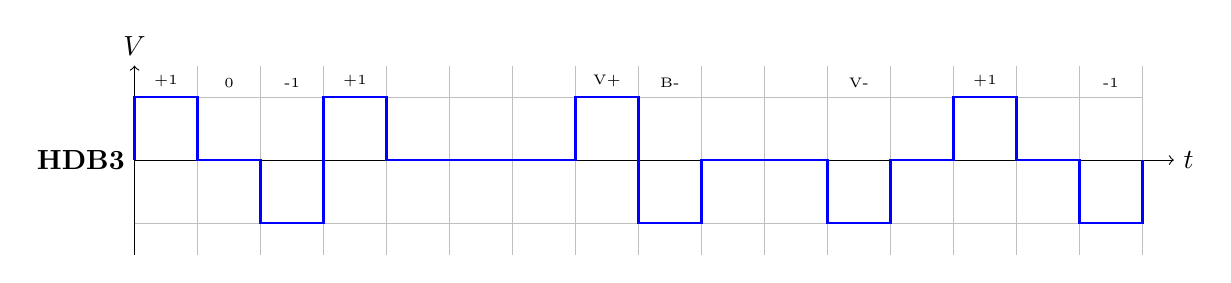
\begin{tikzpicture}[x=0.8cm, y=0.8cm]
        % 绘制网格
        \draw[help lines, step=1, lightgray] (0,-1.5) grid (16,1.5);
        
        % --- HDB3 波形 ---
        \node[left] at (0, 0) {\textbf{HDB3}};
        % 坐标轴
        \draw[->] (0,0) -- (16.5,0) node[right] {$t$};
        \draw[->] (0,-1.5) -- (0,1.5) node[above] {$V$};
        
        % 波形数据: +1 0 -1 +1 0 0 0 +1 -1 0 0 -1 0 +1 0 -1
        \draw[blue, thick] 
            (0,0) -- (0,1) -- (1,1) -- (1,0) -- (2,0) % +1, 0
            -- (2,-1) -- (3,-1) -- (3,0) -- (3,1) -- (4,1) -- (4,0) % -1, +1
            -- (7,0) -- (7,1) -- (8,1) -- (8,0) % 000+1
            -- (8,-1) -- (9,-1) -- (9,0) -- (11,0) -- (11,-1) -- (12,-1) -- (12,0) % -1 0 0 -1
            -- (13,0) -- (13,1) -- (14,1) -- (14,0) % 0 +1
            -- (15,0) -- (15,-1) -- (16,-1) -- (16,0); % 0 -1
            
        % 标注
        \foreach \x/\txt in {0.5/+1, 1.5/0, 2.5/-1, 3.5/+1, 7.5/V+, 8.5/B-, 11.5/V-, 13.5/+1, 15.5/-1}
            \node[above, font=\tiny] at (\x, 1) {\txt};
            
    \end{tikzpicture}
    \end{center}
    \small *注：图中 V+ 表示破坏点，B- 表示调节脉冲。


\noindent \textbf{6-11} 设基带传输系统的发送滤波器、信道及接收滤波器组成的总特性为 $H(\omega)$，若要求以 $2/T_B$ 波特的速率进行数据传输，验证图 P6-5 所示的各种 $H(\omega)$ 能否满足抽样点上无码间串扰的条件？

\begin{figure}[h]
\centering
\begin{tikzpicture}[>=stealth, scale=0.7]
    % --- 图(a) ---
    \begin{scope}[xshift=0cm]
        \draw[->] (-2.5,0) -- (2.5,0) node[right] {\small $\omega$};
        \draw[->] (0,0) -- (0,2.2) node[right] {\scriptsize $H(\omega)$};
        \draw[thick] (-1.2,0) -- (-1.2,1.6) -- (1.2,1.6) -- (1.2,0);
        \node[above left] at (0, 1.6) {\scriptsize 1};
        \node[right] at (1.2, 1.8) {\scriptsize 矩形};
        \node[below] at (-1.2,0) {\scriptsize $-\pi/T_B$};
        \node[below] at (0,0) {\scriptsize 0};
        \node[below] at (1.2,0) {\scriptsize $\pi/T_B$};
        \node at (0,-1.2) {\small (a)};
    \end{scope}

    % --- 图(b) ---
    \begin{scope}[xshift=8cm]
        \draw[->] (-3,0) -- (3,0) node[right] {\small $\omega$};
        \draw[->] (0,0) -- (0,2.2) node[right] {\scriptsize $H(\omega)$};
        \draw[thick] (-2,0) -- (-2,1.6) -- (2,1.6) -- (2,0);
        \node[above left] at (0, 1.6) {\scriptsize 1};
        \node[right] at (2, 1.8) {\scriptsize 矩形};
        \node[below] at (-2,0) {\scriptsize $-3\pi/T_B$};
        \node[below] at (0,0) {\scriptsize 0};
        \node[below] at (2,0) {\scriptsize $3\pi/T_B$};
        \node at (0,-1.2) {\small (b)};
    \end{scope}

    % --- 图(c) ---
    \begin{scope}[xshift=0cm, yshift=-4.5cm]
        \draw[->] (-3.5,0) -- (3.5,0) node[right] {\small $\omega$};
        \draw[->] (0,0) -- (0,2.2) node[right] {\scriptsize $H(\omega)$};
        \draw[thick] (-2.8,0) -- (0,1.6) -- (2.8,0);
        \node[above left] at (0, 1.6) {\scriptsize 1};
        \node[below] at (-2.8,0) {\scriptsize $-4\pi/T_B$};
        \node[below] at (0,0) {\scriptsize 0};
        \node[below] at (2.8,0) {\scriptsize $4\pi/T_B$};
        \node at (0,-1.2) {\small (c)};
    \end{scope}

    % --- 图(d) ---
    \begin{scope}[xshift=8cm, yshift=-4.5cm]
        \draw[->] (-3,0) -- (3,0) node[right] {\small $\omega$};
        \draw[->] (0,0) -- (0,2.2) node[right] {\scriptsize $H(\omega)$};
        \draw[thick, domain=-2.2:2.2, samples=100] plot (\x, {1.6*(1 + cos(\x*180/2.2))/2});
        \node[above left] at (0, 1.6) {\scriptsize 1};
        \node[right] at (1.2, 1.8) {\scriptsize 升余弦型};
        \node[below] at (-2.2,0) {\scriptsize $-2\pi/T_B$};
        \node[below] at (0,0) {\scriptsize 0};
        \node[below] at (2.2,0) {\scriptsize $2\pi/T_B$};
        \node at (0,-1.2) {\small (d)};
    \end{scope}
\end{tikzpicture}
\caption*{对应6-11}
\end{figure}
% --- 答题框 ---
\begin{tcolorbox}[colback=white, colframe=blue!50!black, title=\textbf{题目解答：6-11 验证无码间串扰 (ISI) 条件}]

    \section*{一、 核心公式与判决依据}
    
    要验证系统传输特性 $H(\omega)$ 是否满足无码间串扰条件，需使用频域上的**奈奎斯特第一准则**。
    
    \textbf{1. 奈奎斯特第一准则 (频域公式)：}
    \begin{equation}
        \sum_{k=-\infty}^{\infty} H\left(\omega - k \frac{2\pi}{T_s}\right) = \text{常数}
    \end{equation}
    即：将频谱 $H(\omega)$ 以 $\frac{2\pi}{T_s}$ 为周期进行搬移并叠加，若结果为常数，则无码间串扰。
    
    \textbf{2. 关键参数计算：}
    \begin{itemize}
        \item \textbf{给定传输速率}：$R_B = \frac{2}{T_B}$ (波特/秒)。
        \item \textbf{符号间隔}：$T_s = \frac{1}{R_B} = \frac{T_B}{2}$。
        \item \textbf{频谱搬移周期 (采样角频率)}：
            \begin{equation}
                \omega_s = \frac{2\pi}{T_s} = \frac{2\pi}{T_B / 2} = \frac{4\pi}{T_B}
            \end{equation}
    \end{itemize}
    
    \textbf{判决方法：}
    我们需要检查将各图中的 $H(\omega)$ 每隔 $\frac{4\pi}{T_B}$ 搬移一次并叠加，看总谱是否平坦。
    \end{tcolorbox}

    \section*{二、 逐图验证步骤}
    
    \textbf{搬移周期：$\Omega = \frac{4\pi}{T_B}$}
    
    \textbf{(a) 矩形谱，截止频率 $\pi/T_B$}
    \begin{itemize}
        \item \textbf{分析}：$H(\omega)$ 仅在 $[-\frac{\pi}{T_B}, \frac{\pi}{T_B}]$ 有值。
        \item \textbf{搬移}：
            \begin{itemize}
                \item $k=0$ (主谱)：范围 $[-\frac{\pi}{T_B}, \frac{\pi}{T_B}]$。
                \item $k=1$ (右移)：中心在 $\frac{4\pi}{T_B}$，范围 $[\frac{3\pi}{T_B}, \frac{5\pi}{T_B}]$。
            \end{itemize}
        \item \textbf{叠加结果}：在 $\frac{\pi}{T_B}$ 到 $\frac{3\pi}{T_B}$ 之间存在频谱空隙（值为 0）。叠加后不是常数。
        \item \textbf{结论}：\textbf{不能满足}。
    \end{itemize}

    \textbf{(b) 矩形谱，截止频率 $3\pi/T_B$}
    \begin{itemize}
        \item \textbf{分析}：$H(\omega)$ 在 $[-\frac{3\pi}{T_B}, \frac{3\pi}{T_B}]$ 值为 1。
        \item \textbf{搬移}：
            \begin{itemize}
                \item $k=0$：覆盖 $[-\frac{3\pi}{T_B}, \frac{3\pi}{T_B}]$。
                \item $k=1$ (中心 $\frac{4\pi}{T_B}$)：覆盖 $[\frac{\pi}{T_B}, \frac{7\pi}{T_B}]$。
            \end{itemize}
        \item \textbf{叠加结果}：
            \begin{itemize}
                \item 在区间 $[0, \frac{\pi}{T_B}]$：只有 $k=0$ 分量，总和为 1。
                \item 在区间 $[\frac{\pi}{T_B}, \frac{3\pi}{T_B}]$：$k=0$ 和 $k=1$ 重叠，总和为 $1+1=2$。
            \end{itemize}
            总谱起伏（1 和 2 跳变），不平坦。
        \item \textbf{结论}：\textbf{不能满足}。
    \end{itemize}

    \textbf{(c) 三角形谱，截止频率 $4\pi/T_B$}
    \begin{itemize}
        \item \textbf{分析}：$H(\omega)$ 为三角形，范围 $[-\frac{4\pi}{T_B}, \frac{4\pi}{T_B}]$，峰值为 1。
        \item \textbf{搬移}：
            \begin{itemize}
                \item $k=0$：在 $[0, \frac{4\pi}{T_B}]$ 上，函数为直线下降 $1 - \frac{\omega}{4\pi/T_B}$。
                \item $k=1$ (中心 $\frac{4\pi}{T_B}$)：在 $[0, \frac{4\pi}{T_B}]$ 上，函数为直线上升 $\frac{\omega}{4\pi/T_B}$（因为是左半边三角形移到了这里）。
            \end{itemize}
        \item \textbf{叠加结果}：
            $$ \sum = \left(1 - \frac{\omega}{4\pi/T_B}\right) + \frac{\omega}{4\pi/T_B} = 1 $$
            在所有区间叠加后均为常数 1。
        \item \textbf{结论}：\textbf{能满足}。
    \end{itemize}

    \textbf{(d) 升余弦型，截止频率 $2\pi/T_B$}
    \begin{itemize}
        \item \textbf{分析}：$H(\omega)$ 范围 $[-\frac{2\pi}{T_B}, \frac{2\pi}{T_B}]$。
        \item \textbf{搬移}：
            \begin{itemize}
                \item $k=0$：结束于 $\frac{2\pi}{T_B}$。
                \item $k=1$ (中心 $\frac{4\pi}{T_B}$)：开始于 $\frac{4\pi}{T_B} - \frac{2\pi}{T_B} = \frac{2\pi}{T_B}$。
            \end{itemize}
        \item \textbf{叠加结果}：两段频谱只是在 $\frac{2\pi}{T_B}$ 处相切，并没有通过“互补”重叠成一条直线。总谱依然呈现波浪状（馒头波形）。
        \item \textbf{结论}：\textbf{不能满足}。
    \end{itemize}

\vspace{1em}

\noindent \textbf{6-12} 欲以 $R_B = 10^3$ 波特的速率传输数字基带信号，试问采用图 P6-6 中的哪一种传输特性较好？并简要说明其理由。

\begin{figure}[h]
\centering
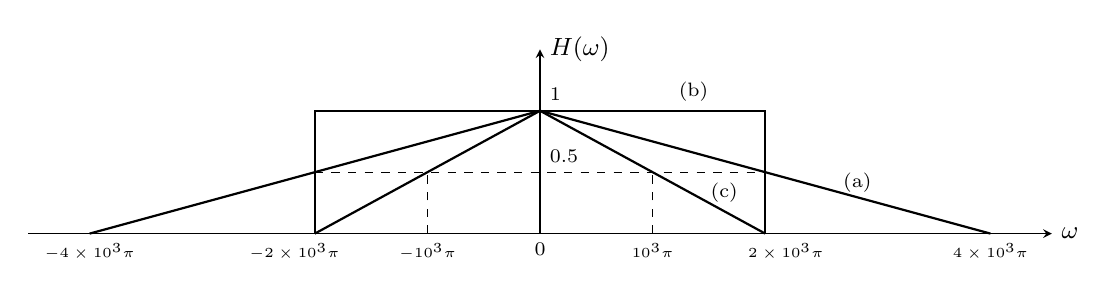
\begin{tikzpicture}[>=stealth, scale=1.3]
    % --- 坐标轴 ---
    \draw[->] (-5, 0) -- (5, 0) node[right] {\small $\omega$};
    \draw[->] (0, 0) -- (0, 1.8) node[right] {\small $H(\omega)$};

    % --- 垂直刻度 ---
    \node[above right] at (0, 1.2) {\scriptsize 1};
    \node[above right] at (0, 0.6) {\scriptsize 0.5};

    % --- 绘制曲线 ---
    % (b) 矩形
    \draw[thick] (-2.2, 0) -- (-2.2, 1.2) -- (2.2, 1.2) -- (2.2, 0);
    \node[above] at (1.5, 1.2) {\scriptsize (b)};

    % (a) 宽三角形
    \draw[thick] (-4.4, 0) -- (0, 1.2) -- (4.4, 0);
    \node at (3.1, 0.5) {\scriptsize (a)};

    % (c) 窄三角形
    \draw[thick] (-2.2, 0) -- (0, 1.2) -- (2.2, 0);
    \node at (1.8, 0.4) {\scriptsize (c)};

    % --- 辅助虚线 ---
    \draw[dashed] (-2.2, 0.6) -- (2.2, 0.6);
    \draw[dashed] (1.1, 0) -- (1.1, 0.6);
    \draw[dashed] (-1.1, 0) -- (-1.1, 0.6);
    \draw[dashed] (2.2, 0) -- (2.2, 0.6);
    \draw[dashed] (-2.2, 0) -- (-2.2, 0.6);

    % --- X轴标签 ---
    \node[below] at (0, 0) {\scriptsize 0};
    \node[below] at (1.1, 0) {\tiny $10^3\pi$};
    \node[below] at (2.4, 0) {\tiny $2 \times 10^3\pi$};
    \node[below] at (4.4, 0) {\tiny $4 \times 10^3\pi$};
    \node[below] at (-1.1, 0) {\tiny $-10^3\pi$};
    \node[below] at (-2.4, 0) {\tiny $-2 \times 10^3\pi$};
    \node[below] at (-4.4, 0) {\tiny $-4 \times 10^3\pi$};
\end{tikzpicture}
\caption*{对应6-12 图P6-6}
\end{figure}
% --- 答题框 ---
\begin{tcolorbox}[colback=white, colframe=blue!50!black, title=\textbf{题目解答：6-12 最佳基带传输特性的选择}]

    \section*{一、 核心公式与判决准则}
    
    \textbf{1. 奈奎斯特角频率 (Nyquist Frequency)：}
    对于给定的码元传输速率 $R_B$ (Baud)，系统传输的最小理论带宽（奈奎斯特带宽）对应的角频率为：
    \begin{equation}
        \omega_N = \frac{\omega_s}{2} = \frac{2\pi R_B}{2} = \pi R_B
    \end{equation}
    
    \textbf{2. 奈奎斯特第一准则 (频域对称性)：}
    为了实现无码间串扰 (Zero ISI)，传输特性 $H(\omega)$ 的边沿必须关于截止频率点 $(\omega_N, 0.5)$ 呈奇对称 (斜对称)。即满足：
    \begin{equation}
        H(\omega_N - \Delta \omega) + H(\omega_N + \Delta \omega) = 1
    \end{equation}
    
    \textbf{3. 物理可实现性评价：}
    \begin{itemize}
        \item \textbf{尾部衰减}：频带越宽（滚降系数 $\alpha$ 越大），时域波形 $h(t)$ 的尾部衰减越快（如 $1/t^2$ 或 $1/t^3$），对定时抖动越不敏感。
        \item \textbf{滤波器实现}：边缘平滑的特性比垂直截止的特性更容易用模拟滤波器实现。
    \end{itemize}

    \end{tcolorbox}

    \section*{二、 具体分析步骤}
    
    \textbf{1. 确定本题的关键频率点}
    
    已知传输速率 $R_B = 10^3$ Baud。
    计算奈奎斯特角频率：
    \begin{equation}
        \omega_N = \pi R_B = \pi \times 10^3 \text{ rad/s}
    \end{equation}
    这意味着，我们选择的 $H(\omega)$ 必须在 $\omega = 10^3\pi$ 处满足**幅度为 0.5** 且**关于该点奇对称**。
    
    \textbf{2. 逐一分析三个特性}
    
    \begin{itemize}
        \item \textbf{特性 (a) [大三角形]}：
            \begin{itemize}
                \item 截止频率为 $4\times 10^3\pi$。
                \item 在关键点 $\omega_N = 10^3\pi$ 处，由相似三角形可知其幅度为 $H(\omega_N) = 0.75$（因为 $1000/4000 = 1/4$ 处，幅度降了 $1/4$）。
                \item \textbf{结论}：$0.75 \neq 0.5$，不满足对称条件，\textbf{存在严重的码间串扰}。
            \end{itemize}
            
        \item \textbf{特性 (b) [矩形谱]}：
            \begin{itemize}
                \item 截止频率为 $2\times 10^3\pi$。
                \item 在关键点 $\omega_N = 10^3\pi$ 处，幅度恒为 1。
                \item 即使我们假设它是一个截止频率恰好为 $\pi \times 10^3$ 的理想低通滤波器（图上看起来像宽带），其时域波形为 Sinc 函数 ($\frac{\sin t}{t}$)，尾部衰减慢 ($1/t$)，对定时误差极为敏感，且物理上无法制造出边缘如此陡峭的滤波器。
                \item \textbf{结论}：\textbf{物理可实现性差，且容易产生码间串扰}。
            \end{itemize}
            
        \item \textbf{特性 (c) [直线滚降/升余弦]}：
            \begin{itemize}
                \item 截止频率为 $2\times 10^3\pi$。
                \item 这是一个线性滚降特性。观察图像，连接 $(0,1)$ 和 $(2\times 10^3\pi, 0)$ 的直线，其中点坐标恰好是 $(\mathbf{10^3\pi, 0.5})$。
                \item \textbf{结论}：
                    \begin{enumerate}
                        \item \textbf{满足准则}：该特性关于 $(\omega_N, 0.5)$ 严格奇对称，因此\textbf{无码间串扰}。
                        \item \textbf{性能优良}：这是滚降系数 $\alpha=1$ 的升余弦滚降特性。相比矩形谱，它的时域尾部衰减速度快 ($1/t^3$ 对于线性滚降，或 $1/t^2$ 视具体近似)，\textbf{对定时抖动不敏感}。
                    \end{enumerate}
            \end{itemize}
    \end{itemize}

    \paragraph{最终结论：}
    \textbf{应采用特性 (c)}。
    \newline
    \textbf{理由}：只有特性 (c) 在满足 $R_B=10^3$ Baud 的无码间串扰条件（关于 $10^3\pi$ 奇对称）的同时，具有平滑的边缘，易于物理实现，且时域波形衰减快，抗定时抖动性能最好。

\vspace{1em}

\noindent \textbf{【思考题】}

\begin{enumerate}
    \item 在数字基带系统中造成误码的原因是什么？请分析原因并给出减少误码的有效解决办法。
    \item 请画出第 IV 类部分响应系统组成框图。
\end{enumerate}

\vspace{2em}

\noindent \textbf{【思考题答案】}

\begin{enumerate}
    \item 在数字基带系统中造成误码的原因是什么？请分析原因并给出减少误码的有效解决办法。\\
    \textbf{答：} 
    \begin{itemize}
        \item \textbf{原因：} 
            \begin{enumerate}
                \item 噪声：信道中的加性高斯白噪声等；
                \item 码间串扰：由于信道不理想或带宽限制导致；
                \item 信道失真：频率选择性衰落、多径效应等；
                \item 同步误差：位同步、帧同步不准确；
                \item 判决门限漂移：接收机电路不稳定。
            \end{enumerate}
        \item \textbf{解决办法：}
            \begin{enumerate}
                \item 采用均衡技术（如时域均衡器）消除码间串扰；
                \item 选择抗干扰性强的传输码型（如HDB$_3$、AMI等）；
                \item 优化收发滤波器，满足奈奎斯特准则；
                \item 采用同步技术提高定时精度；
                \item 应用差错控制编码（如线性分组码、卷积码）和交织技术；
                \item 合理设计判决门限，采用自适应阈值。
            \end{enumerate}
    \end{itemize}

    \item 请画出第 IV 类部分响应系统组成框图。\\
    \textbf{答：} 第 IV 类部分响应系统框图如下：
    \begin{figure}[h]
        \centering
        \begin{tikzpicture}[>=stealth, node distance=1.5cm, auto]
            % 节点
            \node (input) {$a_k$};
            \node[draw, rectangle, right of=input] (precode) {预编码};
            \node[right of=precode] (bk) {$b_k$};
            \node[draw, rectangle, right of=bk] (delay) {$T_s$};
            \node[right of=delay] (bkm1) {$b_{k-1}$};
            \node[draw, circle, right of=bkm1] (sum) {$-$};
            \node[right of=sum] (ck) {$c_k$};
            \node[draw, rectangle, right of=ck] (mod) {$\mod 2$};
            \node[right of=mod] (output) {$\hat{a}_k$};
            % 连接
            \draw[->] (input) -- (precode);
            \draw[->] (precode) -- (bk);
            \draw[->] (bk) -- (delay);
            \draw[->] (delay) -- (bkm1);
            \draw[->] (bk) -- (sum);
            \draw[->] (bkm1) -- (sum);
            \draw[->] (sum) -- (ck);
            \draw[->] (ck) -- (mod);
            \draw[->] (mod) -- (output);
            % 标注
            \node[above of=precode, node distance=1cm] {差分编码};
            \node[above of=sum, node distance=1cm] {相关编码};
            \node[above of=mod, node distance=1cm] {模2判决};
        \end{tikzpicture}
        \caption{第 IV 类部分响应系统框图}
    \end{figure}
    其中，预编码（差分编码）规则：$b_k = a_k \oplus b_{k-1}$，相关编码：$c_k = b_k - b_{k-1}$，模2判决：$\hat{a}_k = c_k \mod 2$。
\end{enumerate}

\mysection{第七章}

\begin{enumerate}[label=\textbf{7-\arabic*}]
    \item 设发送的二进制信息序列为 1011001，码元速率为 2000 Baud，载波信号为 $\sin(8\pi \times 10^3 t)$。试确定：
    \begin{enumerate}
        \item 每个码元中包含多少个载波周期？
        \item 画出 OOK、2PSK 及 2DPSK 信号的波形，并注意观察其波形各有什么特点。
        \item 计算 2ASK、2PSK、2DPSK 信号的第一谱零点带宽。
    \end{enumerate}
    % --- 答题框 ---
\begin{tcolorbox}[colback=white, colframe=blue!50!black, title=\textbf{题目解答：7-1 二进制数字调制系统分析}]

    \section*{一、 核心公式与原理}
    
    \textbf{1. 载波周期数计算：}
    \begin{itemize}
        \item 载波频率 $f_c = \frac{\omega_c}{2\pi}$
        \item 码元宽度 $T_B = \frac{1}{R_B}$
        \item 每个码元的周期数 $N = f_c \times T_B$
    \end{itemize}
    
    \textbf{2. 第一谱零点带宽 (First Null-to-Null Bandwidth)：}
    对于矩形脉冲调制的数字信号，其功率谱主瓣宽度（第一谱零点带宽）$B$ 取决于码元速率 $R_B$：
    \begin{equation}
        B_{2ASK} = B_{2PSK} = B_{2DPSK} = 2 R_B
    \end{equation}
    *(注：这里指双边带带宽)*
    
    \textbf{3. 调制规则：}
    \begin{itemize}
        \item \textbf{OOK (2ASK)}: 1 $\rightarrow$ 发送载波；0 $\rightarrow$ 不发送载波。
        \item \textbf{2PSK}: 1 $\rightarrow$ 0 相位 ($\sin \omega t$)；0 $\rightarrow$ $\pi$ 相位 ($-\sin \omega t$)。*(规则可选，本题按此绘制)*
        \item \textbf{2DPSK}: 利用前后码元的相位变化来传递信息。
            \begin{itemize}
                \item 编码规则（差分码）：$b_n = a_n \oplus b_{n-1}$。
                \item 假设初始参考位为 1，且输入“1”代表相位翻转，“0”代表相位不变。
            \end{itemize}
    \end{itemize}

    \end{tcolorbox}


    \section*{二、 具体计算步骤}
    
    \textbf{(a) 计算每个码元中包含的载波周期数}
    
    已知载波信号 $\sin(8\pi \times 10^3 t)$，码元速率 $R_B = 2000$ Baud。
    \begin{enumerate}
        \item \textbf{载波频率}：
            $$ \omega_c = 8\pi \times 10^3 \implies f_c = 4000 \text{ Hz} $$
        \item \textbf{码元宽度}：
            $$ T_B = \frac{1}{2000} = 0.5 \times 10^{-3} \text{ s} = 0.5 \text{ ms} $$
        \item \textbf{周期数}：
            $$ N = f_c \times T_B = 4000 \times \frac{1}{2000} = \mathbf{2} $$
    \end{enumerate}
    即每个码元包含 \textbf{2 个完整的正弦波周期}。
    
    \vspace{0.5cm}
    
    \textbf{(c) 计算第一谱零点带宽}
    
    对于 2ASK、2PSK 和 2DPSK，若采用矩形脉冲，其带宽计算公式相同：
    $$ B = 2 R_B $$
    代入数值：
    $$ B = 2 \times 2000 = \mathbf{4000 \text{ Hz}} $$

    \hrulefill
    
    \section*{三、 波形绘制 (b)}
    
    \textbf{输入序列：} $1 \quad 0 \quad 1 \quad 1 \quad 0 \quad 0 \quad 1$
    
    \textbf{1. 2DPSK 差分编码预处理：}
    设初始参考位 $b_{-1}=1$。规则：$a_n=1$ 则翻转，$a_n=0$ 则不变 ($b_n = a_n \oplus b_{n-1}$)。
    \begin{itemize}
        \item $a_0=1 \to b_0 = 1 \oplus 1 = 0$
        \item $a_1=0 \to b_1 = 0 \oplus 0 = 0$
        \item $a_2=1 \to b_2 = 1 \oplus 0 = 1$
        \item $a_3=1 \to b_3 = 1 \oplus 1 = 0$
        \item $a_4=0 \to b_4 = 0 \oplus 0 = 0$
        \item $a_5=0 \to b_5 = 0 \oplus 0 = 0$
        \item $a_6=1 \to b_6 = 1 \oplus 0 = 1$
    \end{itemize}
    \textbf{DPSK 相对码序列：} $0 \ 0 \ 1 \ 0 \ 0 \ 0 \ 1$ (后续按此序列进行 PSK 调制)
    
    \vspace{0.5cm}
    
    \begin{center}
    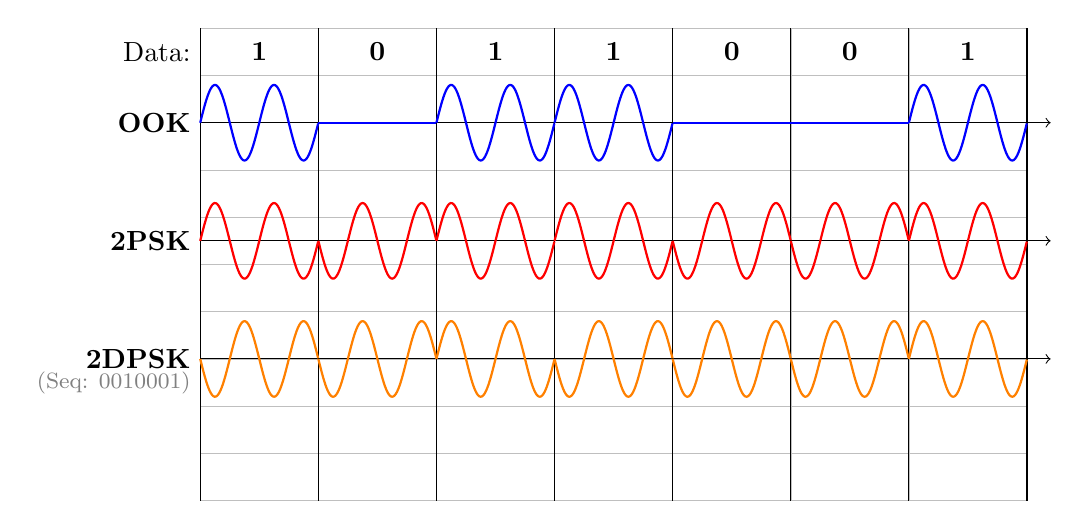
\begin{tikzpicture}[x=1.5cm, y=0.6cm]
        % 网格与坐标
        \draw[help lines, step=1, lightgray] (0,-9) grid (7,1);
        \foreach \x in {0,1,...,7} \draw (\x, 1) -- (\x, -9);
        
        % 顶部标注序列
        \node[left] at (0, 0.5) {Data:};
        \foreach \x/\val in {0.5/1, 1.5/0, 2.5/1, 3.5/1, 4.5/0, 5.5/0, 6.5/1}
            \node at (\x, 0.5) {\textbf{\val}};

        % --- OOK 波形 ---
        \node[left] at (0, -1) {\textbf{OOK}};
        \draw[->] (0,-1) -- (7.2,-1);
        % 1:有波, 0:无波
        \draw[blue, thick, samples=100, domain=0:1] plot (\x, {-1 + 0.8*sin(720*\x)}); % 1
        \draw[blue, thick] (1,-1) -- (2,-1); % 0
        \draw[blue, thick, samples=100, domain=2:3] plot (\x, {-1 + 0.8*sin(720*(\x-2))}); % 1
        \draw[blue, thick, samples=100, domain=3:4] plot (\x, {-1 + 0.8*sin(720*(\x-3))}); % 1
        \draw[blue, thick] (4,-1) -- (6,-1); % 0 0
        \draw[blue, thick, samples=100, domain=6:7] plot (\x, {-1 + 0.8*sin(720*(\x-6))}); % 1
        
        % --- 2PSK 波形 ---
        \node[left] at (0, -3.5) {\textbf{2PSK}};
        \draw[->] (0,-3.5) -- (7.2,-3.5);
        % 1:正相, 0:反相 (sin(x+180) = -sin(x))
        \draw[red, thick, samples=100, domain=0:1] plot (\x, {-3.5 + 0.8*sin(720*\x)}); % 1
        \draw[red, thick, samples=100, domain=1:2] plot (\x, {-3.5 + 0.8*sin(720*\x + 180)}); % 0
        \draw[red, thick, samples=100, domain=2:3] plot (\x, {-3.5 + 0.8*sin(720*\x)}); % 1
        \draw[red, thick, samples=100, domain=3:4] plot (\x, {-3.5 + 0.8*sin(720*\x)}); % 1
        \draw[red, thick, samples=100, domain=4:5] plot (\x, {-3.5 + 0.8*sin(720*\x + 180)}); % 0
        \draw[red, thick, samples=100, domain=5:6] plot (\x, {-3.5 + 0.8*sin(720*\x + 180)}); % 0
        \draw[red, thick, samples=100, domain=6:7] plot (\x, {-3.5 + 0.8*sin(720*\x)}); % 1

        % --- 2DPSK 波形 ---
        \node[left] at (0, -6) {\textbf{2DPSK}};
        \node[left, font=\footnotesize, gray] at (0, -6.5) {(Seq: 0010001)};
        \draw[->] (0,-6) -- (7.2,-6);
        % 序列 0 0 1 0 0 0 1 (0为反相, 1为正相)
        % 注意：这里直接画出相对码对应的 PSK 波形
        \draw[orange, thick, samples=100, domain=0:1] plot (\x, {-6 + 0.8*sin(720*\x + 180)}); % 0
        \draw[orange, thick, samples=100, domain=1:2] plot (\x, {-6 + 0.8*sin(720*\x + 180)}); % 0
        \draw[orange, thick, samples=100, domain=2:3] plot (\x, {-6 + 0.8*sin(720*\x)});       % 1
        \draw[orange, thick, samples=100, domain=3:4] plot (\x, {-6 + 0.8*sin(720*\x + 180)}); % 0
        \draw[orange, thick, samples=100, domain=4:5] plot (\x, {-6 + 0.8*sin(720*\x + 180)}); % 0
        \draw[orange, thick, samples=100, domain=5:6] plot (\x, {-6 + 0.8*sin(720*\x + 180)}); % 0
        \draw[orange, thick, samples=100, domain=6:7] plot (\x, {-6 + 0.8*sin(720*\x)});       % 1

    \end{tikzpicture}
    \end{center}
    
    \textbf{波形特点观察：}
    \begin{itemize}
        \item \textbf{OOK}：有载波表示“1”，无载波表示“0”，包络起伏大。
        \item \textbf{2PSK}：振幅恒定，但在码元切换处（如 1$\to$0 或 0$\to$1）相位发生 $180^\circ$ 跳变。
        \item \textbf{2DPSK}：波形与 2PSK 类似，但相位跳变的位置取决于“原数据是否为 1”。例如第 1 个码元数据为 1，则 2DPSK 波形相对于参考相位发生了翻转。
    \end{itemize}

    \item 设某 2FSK 调制系统的码元速率为 2000 Baud，已调信号的载频分别为 6000Hz (对应“1”码) 和 4000Hz (对应“0”码)。
    \begin{enumerate}
        \item 若发送的信息序列为 1011001，试画出 2FSK 信号的时间波形；
        \item 试画出 2FSK 信号的功率谱密度示意图，并计算 2FSK 信号的第一谱零点带宽。
        \item 讨论应选择什么解调方法解调该 2FSK 信号。
    \end{enumerate}
% --- 答题框 ---
\begin{tcolorbox}[colback=white, colframe=blue!50!black, title=\textbf{题目解答：7-2 2FSK 系统的波形、带宽与解调}]

    \section*{一、 核心公式与参数分析}
    
    \textbf{1. 信号参数计算：}
    \begin{itemize}
        \item \textbf{码元宽度}：$T_B = \frac{1}{R_B}$。
        \item \textbf{载波周期数}：每个码元内包含的完整正弦波个数 $N = f_c \times T_B$。
    \end{itemize}
    
    \textbf{2. 2FSK 带宽公式 (第一谱零点带宽)：}
    2FSK 信号可以看作是两个不同载频的 ASK 信号的叠加。其频带宽度约为两载频之差加上两个基带带宽：
    \begin{equation}
        B_{2FSK} = |f_2 - f_1| + 2R_B
    \end{equation}
    *(注：这是工程上常用的计算方法，对应两个主瓣覆盖的总范围)*
    
    \textbf{3. 已知条件：}
    \begin{itemize}
        \item $R_B = 2000$ Baud $\Rightarrow T_B = 0.5$ ms。
        \item “1” 码对应 $f_1 = 6000$ Hz。
        \item “0” 码对应 $f_2 = 4000$ Hz。
        \item 输入序列：$1 \ 0 \ 1 \ 1 \ 0 \ 0 \ 1$。
    \end{itemize}

    \end{tcolorbox}    


    \section*{二、 具体计算步骤}
    
    \textbf{(a) 确定每个码元的波形周期}
    
    \begin{itemize}
        \item \textbf{对应“1”码 ($6000$ Hz)}：
            $$ N_1 = f_1 \times T_B = 6000 \times 0.5 \times 10^{-3} = \mathbf{3} \text{ 个周期} $$
        \item \textbf{对应“0”码 ($4000$ Hz)}：
            $$ N_2 = f_2 \times T_B = 4000 \times 0.5 \times 10^{-3} = \mathbf{2} \text{ 个周期} $$
    \end{itemize}
    \textbf{绘图策略}：遇到“1”画 3 个密集波，遇到“0”画 2 个稀疏波。
    
    \textbf{(b) 计算第一谱零点带宽}
    
    代入带宽公式：
    \begin{align*}
        B_{2FSK} &= |6000 - 4000| + 2 \times 2000 \\
                 &= 2000 + 4000 \\
                 &= \mathbf{6000 \text{ Hz}}
    \end{align*}
    
    *频域分布解释：* 
    \begin{itemize}
        \item 低频主瓣中心在 4000 Hz，零点范围 $[4000-2000, 4000+2000] = [2000, 6000]$。
        \item 高频主瓣中心在 6000 Hz，零点范围 $[6000-2000, 6000+2000] = [4000, 8000]$。
        \item 总覆盖范围：$2000 \text{ Hz} \sim 8000 \text{ Hz}$，带宽为 $6000$ Hz。
    \end{itemize}


    
    \section*{三、 图示绘制 (a) \& (b)}
    
    \begin{center}
    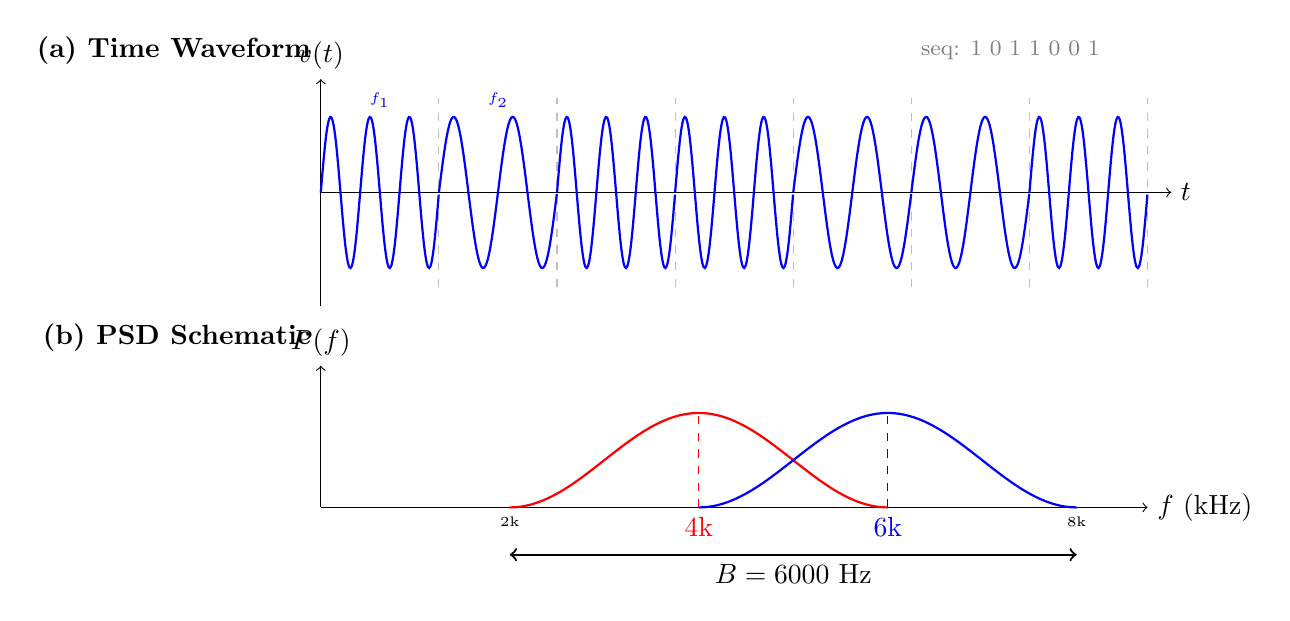
\begin{tikzpicture}[x=1.5cm, y=1.2cm]
    
        % --- (a) 时间波形 ---
        \node[left, font=\bfseries] at (0, 1.5) {(a) Time Waveform};
        \node[right, gray, font=\footnotesize] at (5, 1.5) {seq: 1 0 1 1 0 0 1};
        
        % 坐标轴
        \draw[->] (0,0) -- (7.2,0) node[right] {$t$};
        \draw[->] (0,-1.2) -- (0,1.2) node[above] {$v(t)$};
        
        % 辅助虚线
        \foreach \x in {1,...,7} \draw[dashed, lightgray] (\x, -1) -- (\x, 1);
        
        % 绘制波形: 1(3周期), 0(2周期)
        % 为了波形美观，假设每个码元起始相位为0 (键控切换)
        % 3 cycles = sin(3 * 360 * x) = sin(1080 * x)
        % 2 cycles = sin(2 * 360 * x) = sin(720 * x)
        
        \draw[blue, thick, samples=100, smooth]
            plot[domain=0:1] (\x, {0.8*sin(1080*\x)})    % 1
            plot[domain=1:2] (\x, {0.8*sin(720*(\x-1))}) % 0
            plot[domain=2:3] (\x, {0.8*sin(1080*(\x-2))})% 1
            plot[domain=3:4] (\x, {0.8*sin(1080*(\x-3))})% 1
            plot[domain=4:5] (\x, {0.8*sin(720*(\x-4))}) % 0
            plot[domain=5:6] (\x, {0.8*sin(720*(\x-5))}) % 0
            plot[domain=6:7] (\x, {0.8*sin(1080*(\x-6))});% 1
            
        % 标注频率
        \node[above, font=\tiny, blue] at (0.5, 0.8) {$f_1$};
        \node[above, font=\tiny, blue] at (1.5, 0.8) {$f_2$};

        % --- (b) 功率谱示意图 ---
        \begin{scope}[yshift=-4cm]
            \node[left, font=\bfseries] at (0, 1.8) {(b) PSD Schematic};
            \draw[->] (0,0) -- (7,0) node[right] {$f$ (kHz)};
            \draw[->] (0,0) -- (0,1.5) node[above] {$P(f)$};
            
            % 绘制两个 Sinc 主瓣 (示意)
            % f2=4kHz, f1=6kHz. Rb=2kHz.
            % 4kHz 的主瓣范围: 2~6kHz
            % 6kHz 的主瓣范围: 4~8kHz
            
            % f2 频谱
            \draw[red, thick, smooth, samples=50] plot[domain=2:6] (\x*0.8, {cos(90*(\x-4)/2)^2}); 
            \node[below, red] at (4*0.8, 0) {4k};
            \draw[dashed, red] (4*0.8, 0) -- (4*0.8, 1);
            
            % f1 频谱
            \draw[blue, thick, smooth, samples=50] plot[domain=4:8] (\x*0.8, {cos(90*(\x-6)/2)^2});
            \node[below, blue] at (6*0.8, 0) {6k};
            \draw[dashed, blue] (6*0.8, 0) -- (6*0.8, 1);
            
            % 标注带宽
            \draw[<->, thick] (2*0.8, -0.5) -- (8*0.8, -0.5);
            \node[below] at (5*0.8, -0.5) {$B = 6000$ Hz};
            
            % 标注零点
            \node[below, font=\tiny] at (2*0.8, 0) {2k};
            \node[below, font=\tiny] at (8*0.8, 0) {8k};
        \end{scope}

    \end{tikzpicture}
    \end{center}

    \section*{四、 (c) 解调方法讨论}
    
    对于 2FSK 信号，主要有两种解调方法：
    
    \textbf{1. 包络检波法 (非相干解调)}
    \begin{itemize}
        \item \textbf{原理}：使用两个分别调谐于 $f_1$ 和 $f_2$ 的带通滤波器，后接包络检波器，最后比较两个通道的输出电压大小。
        \item \textbf{优点}：\textbf{电路简单，无需提取载波同步信号}。
        \item \textbf{适用性}：在本题中，两频率间隔 $2000$ Hz 足够大（与码元速率相当），可以较好地分离，且通常 FSK 对相位要求不高，因此\textbf{推荐使用此方法}。
    \end{itemize}
    
    \textbf{2. 相干解调法}
    \begin{itemize}
        \item \textbf{原理}：需要产生两个与发送端同频同相的本地载波，分别与接收信号相乘并积分。
        \item \textbf{特点}：抗噪声性能优于非相干解调，但设备复杂（需要载波同步）。
    \end{itemize}
    
    \textbf{结论}：若无特殊的高抗噪要求，通常选择\textbf{包络检波法}（非相干解调）以降低系统复杂度。

    \setcounter{enumi}{11} % 设置计数器
    \item 已知数字信息为“1”时，发送信号的功率为 $1\text{kW}$，信道损耗为 $60\text{dB}$，接收端解调器输入的噪声功率为 $10^{-4}\text{W}$，试求包络检波 OOK 和相干解调 2PSK 系统的误码率。
    % --- 答题框 ---
\begin{tcolorbox}[colback=white, colframe=blue!50!black, title=\textbf{题目解答：7-12 OOK 与 2PSK 系统误码率计算}]

    \section*{一、 核心公式与参数计算}
    
    \textbf{1. 接收信号功率计算：}
    信道损耗通常以 dB (分贝) 给出，线性功率关系如下：
    \begin{equation}
        P_R = P_T \times 10^{-\frac{L_{dB}}{10}}
    \end{equation}
    其中 $P_T$ 为发送功率，$L_{dB}$ 为信道损耗。
    
    \textbf{2. 信噪比 (SNR) 计算：}
    输入信噪比 $r$ 定义为接收信号功率与噪声功率之比：
    \begin{equation}
        r = \frac{P_R}{P_n}
    \end{equation}
    
    \textbf{3. 误码率 ($P_e$) 公式：}
    \begin{itemize}
        \item \textbf{包络检波 OOK (非相干解调)}：
            在高信噪比条件下，误码率近似公式为：
            \begin{equation}
                P_{e, OOK} \approx \frac{1}{2} e^{-r/4}
            \end{equation}
        \item \textbf{相干解调 2PSK}：
            误码率利用互补误差函数 $\text{erfc}(x)$ 计算：
            \begin{equation}
                P_{e, 2PSK} = \frac{1}{2} \text{erfc}(\sqrt{r})
            \end{equation}
            \footnotesize{*注：有些教材使用 Q 函数表示，即 $Q(\sqrt{2r})$，二者等价。}
    \end{itemize}

    \end{tcolorbox}

    \section*{二、 具体计算步骤}
    
    \textbf{Step 1: 计算接收端信号功率 $P_R$}
    
    已知：发送功率 $P_T = 1 \text{ kW} = 10^3 \text{ W}$，信道损耗 $L = 60 \text{ dB}$。
    \begin{align*}
        P_R &= 10^3 \times 10^{-\frac{60}{10}} \\
            &= 10^3 \times 10^{-6} \\
            &= \mathbf{10^{-3} \text{ W}}
    \end{align*}
    
    \textbf{Step 2: 计算输入信噪比 $r$}
    
    已知：接收端噪声功率 $P_n = 10^{-4} \text{ W}$。
    \begin{align*}
        r &= \frac{P_R}{P_n} \\
          &= \frac{10^{-3}}{10^{-4}} \\
          &= \mathbf{10}
    \end{align*}
    即信噪比为 10 (或 10dB)。
    
    \textbf{Step 3: 计算包络检波 OOK 的误码率}
    
    将 $r=10$ 代入 OOK 误码率公式：
    \begin{align*}
        P_{e, OOK} &\approx \frac{1}{2} e^{-10/4} \\
                   &= 0.5 \times e^{-2.5} \\
                   &\approx 0.5 \times 0.08208 \\
                   &\approx \mathbf{4.1 \times 10^{-2}}
    \end{align*}
    
    \textbf{Step 4: 计算相干解调 2PSK 的误码率}
    
    将 $r=10$ 代入 2PSK 误码率公式：
    \begin{align*}
        P_{e, 2PSK} &= \frac{1}{2} \text{erfc}(\sqrt{10}) \\
                    &= \frac{1}{2} \text{erfc}(3.162)
    \end{align*}
    查误差函数表或使用近似公式 $\text{erfc}(x) \approx \frac{e^{-x^2}}{x\sqrt{\pi}}$：
    \begin{align*}
        \text{erfc}(3.162) &\approx 7.9 \times 10^{-6} \\
        P_{e, 2PSK} &\approx \frac{1}{2} \times 7.9 \times 10^{-6} \\
                    &\approx \mathbf{3.95 \times 10^{-6}}
    \end{align*}

    \paragraph{结论分析：}
    在相同的信噪比 ($r=10$) 下，相干解调 2PSK 的误码率 ($10^{-6}$ 数量级) 远低于非相干 OOK 的误码率 ($10^{-2}$ 数量级)。这体现了相干解调与 PSK 调制方式在抗噪声性能上的显著优势。


\end{enumerate}

\noindent\textbf{【思考题】}
\begin{enumerate}
    \item 试比较四种二进制数字调制系统的频带宽度、频带利用率和误码率。
    \item 二进制数字调制系统的误码率与哪些因素有关？如何提高系统的可靠性？
\end{enumerate}

\noindent\textbf{【思考题答案】}
\begin{enumerate}
    \item 四种二进制数字调制系统的比较：
        \begin{itemize}
            \item \textbf{频带宽度}：
                \begin{itemize}
                    \item 2ASK 和 2PSK（包括 2DPSK）：第一谱零点带宽为 $2R_B$，其中 $R_B$ 为码元速率。
                    \item 2FSK：带宽约为 $|f_1 - f_2| + 2R_B$，通常大于 2ASK 和 2PSK。
                \end{itemize}
            \item \textbf{频带利用率}（单位带宽传输的码元速率）：
                \begin{itemize}
                    \item 2ASK 和 2PSK：理论最大为 $1$ Baud/Hz，但实际由于需要带宽 $2R_B$，所以利用率约为 $0.5$ Baud/Hz。
                    \item 2FSK：由于带宽较宽，频带利用率较低，通常小于 $0.5$ Baud/Hz。
                \end{itemize}
            \item \textbf{误码率}（在相同信噪比条件下，从好到差排列）：
                \begin{itemize}
                    \item 相干解调 2PSK 误码率最低。
                    \item 相干解调 2DPSK（实际采用差分相干解调时，性能略差于相干 2PSK）。
                    \item 相干解调 2ASK 和 2FSK 误码率相近，但 2ASK 对门限敏感。
                    \item 非相干解调（包络检波）性能差于相干解调，其中非相干 2FSK 优于非相干 2ASK。
                \end{itemize}
        \end{itemize}

    \item 二进制数字调制系统的误码率主要与以下因素有关：
        \begin{itemize}
            \item \textbf{信噪比}：信噪比越高，误码率越低。
            \item \textbf{调制方式}：在相同信噪比下，2PSK 抗噪声性能最好，2FSK 次之，2ASK 最差。
            \item \textbf{解调方式}：相干解调比非相干解调性能好，但设备复杂。
            \item \textbf{信道特性}：如多径、衰落等会影响误码率。
            \item \textbf{码间串扰}：若带宽有限或传输特性不理想，会引起码间串扰，增加误码率。
        \end{itemize}
        提高系统可靠性的方法：
        \begin{itemize}
            \item 增加发送功率以提高信噪比。
            \item 选择抗噪声性能好的调制解调方式，如 2PSK 相干解调。
            \item 采用差错控制编码（信道编码）来检错和纠错。
            \item 改善信道特性，如采用均衡技术消除码间串扰。
            \item 采用分集技术、自适应技术等对抗衰落。
        \end{itemize}
\end{enumerate}

\mysection{第八章}
\noindent \textbf{8-1} 已知 4PSK 系统的传输速率为 $2400\,\text{b/s}$，试问：

\begin{enumerate}[label=(\arabic*)]
    \item 4PSK 信号的谱零点带宽和频带利用率 ($\text{b}/(\text{s}\cdot\text{Hz})$)；
    \item 若对基带信号采用 $\alpha = 0.4$ 余弦滚降滤波预处理，再进行 4PSK 调制，这时占用的信道带宽和频带利用率为多大？
    \item 若传输带宽不变，而比特率加倍，则调制方式应作何改变？
\end{enumerate}
% --- 答题框 ---
\begin{tcolorbox}[colback=white, colframe=blue!50!black, title=\textbf{题目解答：8-1 4PSK 系统的带宽与频带利用率}]

    \section*{一、 核心公式与参数定义}
    
    \textbf{1. 码元速率与比特速率的关系：}
    对于 $M$ 进制调制系统，每个码元携带 $k = \log_2 M$ 比特信息。
    \begin{equation}
        R_B = \frac{R_b}{\log_2 M} \quad (\text{Baud})
    \end{equation}
    其中 $R_B$ 为码元速率 (波特率)，$R_b$ 为信息传输速率 (比特率)。
    
    \textbf{2. 信号带宽计算：}
    \begin{itemize}
        \item \textbf{矩形脉冲 (未整形)}：第一谱零点带宽（双边带）为：
            \begin{equation}
                B_{null} = 2 R_B
            \end{equation}
        \item \textbf{升余弦滚降滤波 (整形后)}：占用频带宽度为：
            \begin{equation}
                B_{\alpha} = R_B (1 + \alpha)
            \end{equation}
            其中 $\alpha$ 为滚降系数。
    \end{itemize}
    
    \textbf{3. 频带利用率：}
    衡量单位带宽内传输的比特数：
    \begin{equation}
        \eta = \frac{R_b}{B} \quad (\text{b/(s}\cdot\text{Hz)})
    \end{equation}

    \end{tcolorbox}

    \section*{二、 具体计算步骤}
    
    \textbf{已知条件：}
    \begin{itemize}
        \item 调制方式：4PSK $\Rightarrow M=4$。
        \item 比特速率：$R_b = 2400 \text{ b/s}$。
        \item 码元速率：$R_B = \frac{2400}{\log_2 4} = \frac{2400}{2} = \mathbf{1200 \text{ Baud}}$。
    \end{itemize}
    
    \vspace{0.5cm}
    
    \textbf{(1) 计算矩形脉冲下的带宽和利用率}
    
    \textbf{谱零点带宽：}
    \begin{align*}
        B_{null} &= 2 R_B \\
                 &= 2 \times 1200 \\
                 &= \mathbf{2400 \text{ Hz}}
    \end{align*}
    
    \textbf{频带利用率：}
    \begin{align*}
        \eta &= \frac{R_b}{B_{null}} \\
             &= \frac{2400}{2400} \\
             &= \mathbf{1 \text{ b/(s}\cdot\text{Hz)}}
    \end{align*}
    
    \vspace{0.5cm}
    
    \textbf{(2) 采用 $\alpha = 0.4$ 滚降滤波后的带宽和利用率}
    
    \textbf{占用信道带宽：}
    \begin{align*}
        B_{\alpha} &= R_B (1 + \alpha) \\
                   &= 1200 \times (1 + 0.4) \\
                   &= 1200 \times 1.4 \\
                   &= \mathbf{1680 \text{ Hz}}
    \end{align*}
    
    \textbf{频带利用率：}
    \begin{align*}
        \eta_{\alpha} &= \frac{R_b}{B_{\alpha}} \\
                      &= \frac{2400}{1680} \\
                      &\approx \mathbf{1.43 \text{ b/(s}\cdot\text{Hz)}}
    \end{align*}
    
    \vspace{0.5cm}
    
    \textbf{(3) 传输带宽不变，比特率加倍时的调制方式选择}
    
    \textbf{条件分析：}
    \begin{itemize}
        \item \textbf{带宽限制}：保持不变，即 $B_{new} = B_{old}$。
        \item \textbf{新比特率}：$R_b' = 2 R_b = 4800 \text{ b/s}$。
        \item \textbf{假设}：滚降系数 $\alpha$ 保持不变。
    \end{itemize}
    
    \textbf{推导：}
    根据带宽公式 $B = R_B(1+\alpha)$，带宽不变意味着\textbf{码元速率 $R_B$ 必须保持不变}（即仍为 1200 Baud）。
    
    利用公式 $R_b' = R_B \times \log_2 M'$ 计算新的进制数 $M'$：
    \begin{align*}
        4800 &= 1200 \times \log_2 M' \\
        \log_2 M' &= \frac{4800}{1200} \\
        \log_2 M' &= 4 \\
        M' &= 2^4 = 16
    \end{align*}
    
    \textbf{结论：}
    为了在带宽不变的情况下使传输速率加倍，调制方式应由 4PSK 改为 \textbf{16PSK} (或 16QAM)。


\vspace{3em} % 题目间距

\noindent \textbf{8-2} 设发送数字序列为 $+1-1-1-1-1-1-1-1+1$，试画出相应的 MSK 信号相位变化图。若码元速率为 $1000\text{B}$，载频为 $3000\text{Hz}$，试画出此 MSK 信号的波形。
% --- 答题框 ---
\begin{tcolorbox}[colback=white, colframe=blue!50!black, title=\textbf{题目解答：8-2 MSK 信号的相位与波形}]

    \section*{一、 核心公式与原理}
    
    \textbf{1. MSK (Minimum Shift Keying) 定义：}
    MSK 是一种调制指数 $h=0.5$ 的连续相位频移键控 (CPFSK)。
    
    \textbf{2. 相位变化规则 (附加相位)：}
    相对于载波相位的变化 $\phi(t)$ 满足线性规律：
    \begin{itemize}
        \item 输入 \textbf{+1}：相位在 $T_B$ 内线性增加 $\mathbf{+\frac{\pi}{2}}$。
        \item 输入 \textbf{-1}：相位在 $T_B$ 内线性减少 $\mathbf{-\frac{\pi}{2}}$。
    \end{itemize}
    \begin{equation}
        \phi(t) = \phi(t_0) \pm \frac{\pi}{2T_B}(t - t_0)
    \end{equation}
    
    \textbf{3. 频率关系：}
    \begin{itemize}
        \item 载波频率 $f_c$ 对应每个码元 $N_c = f_c T_B$ 个周期。
        \item 发送“+1”时的瞬时频率：$f_H = f_c + \frac{1}{4T_B}$。
        \item 发送“-1”时的瞬时频率：$f_L = f_c - \frac{1}{4T_B}$。
    \end{itemize}

    \end{tcolorbox}


    \section*{二、 具体参数计算}
    
    \textbf{已知条件：}
    \begin{itemize}
        \item 序列：$+1, -1, -1, -1, -1, -1, -1, -1, +1$ (共 9 位)。
        \item 速率 $R_B = 1000 \text{ Baud} \Rightarrow T_B = 1 \text{ ms}$。
        \item 载频 $f_c = 3000 \text{ Hz}$。
    \end{itemize}
    
    \textbf{1. 载波周期数：}
    $$ N_c = f_c \times T_B = 3000 \times 10^{-3} = \mathbf{3} $$
    即每个码元包含 3 个中心载波周期。
    
    \textbf{2. 附加相位轨迹推导 (设初始相位为 0)：}
    \begin{itemize}
        \item $t=1$ (+1): $0 \to +\pi/2$
        \item $t=2$ (-1): $+\pi/2 \to 0$
        \item $t=3$ (-1): $0 \to -\pi/2$
        \item $t=4$ (-1): $-\pi/2 \to -\pi$
        \item $t=5$ (-1): $-\pi \to -3\pi/2$
        \item $t=6$ (-1): $-3\pi/2 \to -2\pi$
        \item ...以此类推
    \end{itemize}

    \hrulefill
    
    \section*{三、 图示绘制}

    \begin{center}
    \begin{tikzpicture}[x=1.2cm, y=1.0cm]
    
        % --- 图1: MSK 附加相位路径图 ---
        \node[anchor=west, font=\bfseries] at (-1, 2.5) {(1) MSK 相位轨迹图 $\phi(t)$};
        
        % 坐标轴
        \draw[->] (0,0) -- (9.5,0) node[right] {$t/T_B$};
        \draw[->] (0,-3.5) -- (0,1.5) node[above] {Phase};
        
        % 网格
        \draw[step=1, help lines, lightgray] (0,-3.5) grid (9, 1);
        \foreach \x in {1,...,9} \node[below, font=\footnotesize] at (\x, 0) {\x};
        
        % Y轴刻度
        \node[left, font=\footnotesize] at (0, 0.5) {$\pi/2$};
        \node[left, font=\footnotesize] at (0, 0) {$0$};
        \node[left, font=\footnotesize] at (0, -0.5) {$-\pi/2$};
        \node[left, font=\footnotesize] at (0, -1) {$-\pi$};
        \node[left, font=\footnotesize] at (0, -1.5) {$-3\pi/2$};
        \node[left, font=\footnotesize] at (0, -2) {$-2\pi$};
        \node[left, font=\footnotesize] at (0, -2.5) {$-5\pi/2$};
        \node[left, font=\footnotesize] at (0, -3) {$-3\pi$};
        
        % 序列标注
        \foreach \x/\val in {0.5/+1, 1.5/-1, 2.5/-1, 3.5/-1, 4.5/-1, 5.5/-1, 6.5/-1, 7.5/-1, 8.5/+1}
            \node[above, blue, font=\footnotesize] at (\x, 0.5) {\val};
            
        % 绘制相位路径 (0.5 unit = pi/2)
        \draw[blue, thick] (0,0) 
            -- (1, 0.5)   % +1 -> +pi/2
            -- (2, 0)     % -1 -> 0
            -- (3, -0.5)  % -1 -> -pi/2
            -- (4, -1.0)  % -1 -> -pi
            -- (5, -1.5)  % -1 -> -3pi/2
            -- (6, -2.0)  % -1 -> -2pi
            -- (7, -2.5)  % -1 -> -5pi/2
            -- (8, -3.0)  % -1 -> -3pi
            -- (9, -2.5); % +1 -> -5pi/2
            
        % --- 图2: MSK 信号波形图 ---
        \begin{scope}[yshift=-7cm]
            \node[anchor=west, font=\bfseries] at (-1, 2.0) {(2) MSK 信号波形 $s(t)$};
            \node[anchor=west, font=\footnotesize, gray] at (-1, 1.5) {(每个码元含 3 个载波周期)};
            
            % 坐标轴
            \draw[->] (0,0) -- (9.5,0) node[right] {$t$};
            \draw[->] (0,-1.2) -- (0,1.2) node[above] {$v$};
            \draw[step=1, help lines, lightgray, dashed] (0,-1) grid (9, 1);
            
            % 绘制原理：
            % 基础频率 3Hz (每单位时间3周期)
            % +1: 频率 3.25Hz (相位 +90度/T)
            % -1: 频率 2.75Hz (相位 -90度/T)
            % 必须保持相位连续
            
            % Bit 1: +1 (Freq 3.25), Start Phase 0
            \draw[red, thick, samples=100, smooth, domain=0:1] plot (\x, {sin(360 * 3.25 * \x)});
            
            % Bit 2: -1 (Freq 2.75), Start Phase match end of Bit 1 (1170 deg = 90 deg)
            % Formula: sin(360 * 2.75 * (x-1) + 90)
            \draw[red, thick, samples=100, smooth, domain=1:2] plot (\x, {sin(360 * 2.75 * (\x-1) + 90)});
            
            % Bit 3: -1, Start Phase match end of Bit 2 (90 + 360*2.75 = 1080 = 0 deg)
            % Formula: sin(360 * 2.75 * (x-2) + 0)
            \draw[red, thick, samples=100, smooth, domain=2:3] plot (\x, {sin(360 * 2.75 * (\x-2) + 0)});
            
            % Bit 4: -1, Start Phase match (0 + 360*2.75 = 990 = 270 = -90 deg)
            \draw[red, thick, samples=100, smooth, domain=3:4] plot (\x, {sin(360 * 2.75 * (\x-3) - 90)});
            
            % 为了简化绘图，只画前 4 个码元示意 (后面重复性高且密集)
            % 补全剩余的 -1 只是为了视觉完整
            \draw[red, thick, samples=100, smooth, domain=4:5] plot (\x, {sin(360 * 2.75 * (\x-4) + 180)}); % Start -180
            
            \node[right, red] at (5, 0) {$\cdots$ (后续类似)};
            
        \end{scope}
    \end{tikzpicture}
    \end{center}
    
    \paragraph{波形分析：}
    \begin{itemize}
        \item 在 $t=0 \sim 1$ (输入+1)，波形频率略高 (3.25个周期)，相位累计增加 $\pi/2$。
        \item 在 $t=1 \sim 2$ (输入-1)，波形频率略低 (2.75个周期)，相位累计减少 $\pi/2$。
        \item 关键点：在 $t=1, 2, 3...$ 等码元交界处，红色波形是\textbf{平滑连接}的，没有相位突变，这正是 MSK (连续相位) 的特点。
    \end{itemize}



\mysection{第九章}
% --- 题目 9-3 ---
\noindent \textbf{9-3} 设 2FSK 信号为
\begin{equation*}
    \begin{cases}
        s_0(t) = A\sin 2\pi f_0 t & 0 \leqslant t \leqslant T \\
        s_1(t) = A\sin 2\pi f_1 t & 0 \leqslant t \leqslant T
    \end{cases}
\end{equation*}
且 $f_0 = 2/T$，$f_1 = 2f_0$，$s_0(t)$ 和 $s_1(t)$ 等概出现。

\begin{enumerate}[label=(\arabic*)]
    \item 试画出其相关接收机原理框图；
    \item 设发送码元 010，试画出接收机各点时间波形；
    \item 设信道高斯白噪声的双边功率谱密度为 $n_0/2 \, (\text{W}/\text{Hz})$，试求该系统的误码率。
\end{enumerate}% --- 答题框 ---
\begin{tcolorbox}[colback=white, colframe=blue!50!black, title=\textbf{题目解答：9-3 2FSK 相关接收机设计与分析}]

    \section*{一、 核心公式与定义}
    
    \textbf{1. 信号正交性条件：}
    相关接收机工作的核心前提是两个信号 $s_0(t)$ and $s_1(t)$ 在码元周期 $T$ 内正交：
    \begin{equation}
        \rho = \int_{0}^{T} s_0(t) s_1(t) dt = 0
    \end{equation}
    
    \textbf{2. 码元能量 $E_b$：}
    对于等概出现的正弦波信号 $A\sin(2\pi f t)$，其码元能量为：
    \begin{equation}
        E_b = \int_{0}^{T} [A\sin(2\pi f t)]^2 dt = \frac{A^2 T}{2}
    \end{equation}
    
    \textbf{3. 相干解调 2FSK 误码率：}
    在加性高斯白噪声 (AWGN) 信道下，对于正交信号的相干检测，误码率为：
    \begin{equation}
        P_e = Q\left( \sqrt{\frac{E_b}{n_0}} \right)
    \end{equation}
    其中 $n_0$ 为单边噪声功率谱密度。

    \end{tcolorbox}
    

    \section*{二、 题目具体验证与分析}
    
    \textbf{1. 正交性验证}
    题目给定 $f_0 = 2/T$ 和 $f_1 = 4/T$。
    \begin{itemize}
        \item 两者频率差 $\Delta f = 2/T$，是 $1/2T$ 的整数倍，满足正交条件。
        \item 物理意义：在时间 $T$ 内，$s_0$ 振荡 2 周，$s_1$ 振荡 4 周。它们的乘积积分在一个周期内相互抵消为 0。
    \end{itemize}
    
    \textbf{结论：} 可以使用双路并行的相关器（乘法器+积分器）进行最佳接收。

    \hrulefill

    \section*{三、 (1) 相关接收机原理框图}
    
    \begin{center}
    \begin{tikzpicture}[node distance=1.5cm, >=stealth, auto]
        % 定义样式
        \tikzstyle{block} = [draw, rectangle, minimum height=1cm, minimum width=1.5cm, align=center]
        \tikzstyle{sum} = [draw, circle, inner sep=1pt]
        \tikzstyle{mult} = [draw, circle, inner sep=0pt, minimum size=0.6cm]
        \tikzstyle{coord} = [coordinate]

        % 节点定义
        \node[coord] (input) {};
        \node[coord, right=1cm of input] (split) {};
        
        % 上支路 (f1)
        \node[mult, above right=0.5cm and 1cm of split] (mult1) {$\times$};
        \node[block, right=1cm of mult1] (int1) {$\int_{0}^{T} dt$};
        \node[above=0.5cm of mult1] (osc1) {$\sin 2\pi f_1 t$};
        \node[right=0.2cm of int1] (y1) {$y_1$};
        
        % 下支路 (f0)
        \node[mult, below right=0.5cm and 1cm of split] (mult0) {$\times$};
        \node[block, right=1cm of mult0] (int0) {$\int_{0}^{T} dt$};
        \node[below=0.5cm of mult0] (osc0) {$\sin 2\pi f_0 t$};
        \node[right=0.2cm of int0] (y0) {$y_0$};
        
        % 判决器
        \node[sum, right=2.5cm of split] (comp) {$-$}; 
        \node[block, right=1cm of comp] (decision) {抽样判决\\$t=T$};
        \node[coord, right=1cm of decision] (output) {};

        % 连线
        \draw[->] (input) node[left]{$s(t)$} -- (split);
        \draw[->] (split) |- (mult1);
        \draw[->] (split) |- (mult0);
        \draw[->] (osc1) -- (mult1);
        \draw[->] (osc0) -- (mult0);
        \draw[->] (mult1) -- (int1);
        \draw[->] (mult0) -- (int0);
        \draw[->] (int1) -| node[pos=0.9, left] {$+$} (comp);
        \draw[->] (int0) -| node[pos=0.9, left] {$-$} (comp);
        \draw[->] (comp) -- (decision);
        \draw[->] (decision) -- (output) node[right]{Data Out};
    \end{tikzpicture}
    \end{center}

    \hrulefill
    
    \section*{四、 (2) 各点波形图 (输入 010)}
    
    输入序列：$0 \rightarrow 1 \rightarrow 0$。对应的频率变化：$f_0 \rightarrow f_1 \rightarrow f_0$。
    
    \begin{center}
    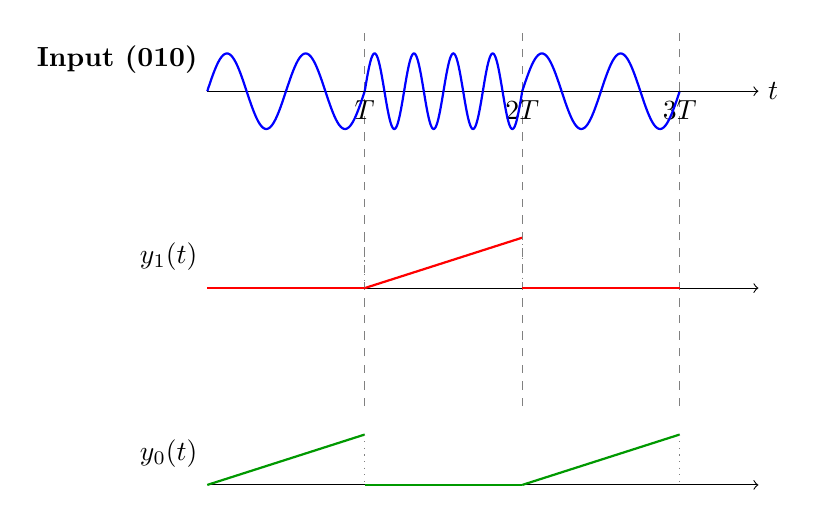
\begin{tikzpicture}[x=2cm, y=0.8cm]
        % 坐标轴
        \draw[->] (0,0) -- (3.5,0) node[right] {$t$};
        \foreach \x in {1, 2, 3} \draw[dashed, gray] (\x, -5) -- (\x, 1);
        \node[below] at (1,0) {$T$}; \node[below] at (2,0) {$2T$}; \node[below] at (3,0) {$3T$};
        
        % 1. 输入信号 s(t)
        \node[left, font=\bfseries] at (0, 0.5) {Input (010)};
        \draw[thick, blue, samples=100, domain=0:1] plot (\x, {0.6*sin(720*\x)});      % f0 (2周)
        \draw[thick, blue, samples=200, domain=1:2] plot (\x, {0.6*sin(1440*(\x-1))}); % f1 (4周)
        \draw[thick, blue, samples=100, domain=2:3] plot (\x, {0.6*sin(720*(\x-2))});  % f0 (2周)
        
        % 2. y1 (f1 支路积分输出)
        \begin{scope}[yshift=-2.5cm]
            \draw[->] (0,0) -- (3.5,0);
            \node[left, font=\bfseries] at (0, 0.5) {$y_1(t)$};
            \draw[thick, red] (0,0) -- (1,0);               % 0: 无响应
            \draw[dotted, gray] (1,0) -- (1,0.8);
            \draw[thick, red] (1,0) -- (2,0.8);             % 1: 积分上升
            \draw[dotted, gray] (2,0.8) -- (2,0);
            \draw[thick, red] (2,0) -- (3,0);               % 0: 无响应
        \end{scope}
        
        % 3. y0 (f0 支路积分输出)
        \begin{scope}[yshift=-5cm]
            \draw[->] (0,0) -- (3.5,0);
            \node[left, font=\bfseries] at (0, 0.5) {$y_0(t)$};
            \draw[thick, green!60!black] (0,0) -- (1,0.8);  % 0: 积分上升
            \draw[dotted, gray] (1,0.8) -- (1,0);
            \draw[thick, green!60!black] (1,0) -- (2,0);    % 1: 无响应
            \draw[thick, green!60!black] (2,0) -- (3,0.8);  % 0: 积分上升
            \draw[dotted, gray] (3,0.8) -- (3,0);
        \end{scope}
    \end{tikzpicture}
    \end{center}

    \hrulefill

    \section*{五、 (3) 误码率计算}
    
    直接利用第一部分的公式：
    \begin{align*}
        P_e &= Q\left( \sqrt{\frac{E_b}{n_0}} \right) \\
            &= Q\left( \sqrt{\frac{A^2 T / 2}{n_0}} \right) \\
            &= \mathbf{Q\left( \sqrt{\frac{A^2 T}{2 n_0}} \right)}
    \end{align*}
    
    \textit{注：此处假设 $n_0/2$ 为双边功率谱密度，即公式中的 $n_0$ 为单边谱密度。}



\vspace{3em} % 题目间距

% --- 题目 9-6 ---
\noindent \textbf{9-6} 设二进制双极性信号最佳传输系统中，信号“0”和“1”是等概率发送的，信号传输速率为 $56\,\text{kb/s}$，接收码元波形为不归零矩形脉冲，信道加性高斯白噪声的双边功率谱密度等于 $10^{-15}\,\text{W}/\text{Hz}$。试问为使误码率不大于 $10^{-5}$，需要的最小接收信号功率等于多少？

% --- 答题框 ---
\begin{tcolorbox}[colback=white, colframe=blue!50!black, title=\textbf{题目解答：9-6 最佳传输系统的最小信号功率计算}]

    \section*{一、 核心公式与参数定义}
    
    \textbf{1. 系统模型：}
    二进制双极性信号 (Bipolar/Antipodal)，即发送 $+A$ 或 $-A$。
    对于加性高斯白噪声 (AWGN) 信道下的最佳接收机（匹配滤波器或相关器），其误码率公式为：
    \begin{equation}
        P_e = Q\left( \sqrt{\frac{2E_b}{n_0}} \right)
    \end{equation}
    或者使用互补误差函数表示：
    \begin{equation}
        P_e = \frac{1}{2} \text{erfc}\left( \sqrt{\frac{E_b}{n_0}} \right)
    \end{equation}
    
    \textbf{2. 关键参数关系：}
    \begin{itemize}
        \item \textbf{信号功率 $S$}：与码元能量 $E_b$ 和传输速率 $R_b$ 的关系为：
            \begin{equation}
                S = E_b \times R_b
            \end{equation}
        \item \textbf{噪声功率谱密度}：题目给出的是\textbf{双边}功率谱密度 $P_n(f) = \frac{n_0}{2}$。
            \begin{itemize}
                \item 单边功率谱密度 $n_0 = 2 \times P_n(f)$。
            \end{itemize}
    \end{itemize}

    \end{tcolorbox}

    \section*{二、 具体计算步骤}
    
    \textbf{Step 1: 确定所需的信噪比 $\frac{E_b}{n_0}$}
    
    已知要求误码率 $P_e \le 10^{-5}$。
    查标准正态分布函数表 (Q函数表) 可知，当 $P_e = 10^{-5}$ 时，自变量 $x$ 需满足：
    $$ Q(x) \le 10^{-5} \Rightarrow x \approx 4.265 $$
    即：
    \begin{align*}
        \sqrt{\frac{2E_b}{n_0}} &\ge 4.265 \\
        \frac{2E_b}{n_0} &\ge (4.265)^2 \approx 18.2 \\
        \frac{E_b}{n_0} &\ge 9.1
    \end{align*}
    这意味着，为了达到 $10^{-5}$ 的误码率，码元能量必须至少是单边噪声功率谱密度的 \textbf{9.1 倍}。
    
    \textbf{Step 2: 处理噪声参数}
    
    题目给出双边功率谱密度为 $10^{-15} \text{ W/Hz}$。
    根据定义 $\frac{n_0}{2} = 10^{-15}$，则单边功率谱密度为：
    $$ n_0 = 2 \times 10^{-15} \text{ W/Hz} $$
    
    \textbf{Step 3: 计算最小接收信号功率 $S$}
    
    已知传输速率 $R_b = 56 \text{ kb/s} = 56 \times 10^3 \text{ b/s}$。
    
    利用 $S = E_b \times R_b$ 和 $E_b = 9.1 n_0$：
    \begin{align*}
        S_{min} &= \left( \frac{E_b}{n_0} \right)_{min} \times n_0 \times R_b \\
                &= 9.1 \times (2 \times 10^{-15}) \times (56 \times 10^3) \\
                &= 18.2 \times 56 \times 10^{-12} \\
                &= 1019.2 \times 10^{-12} \text{ W} \\
                &\approx \mathbf{1.02 \times 10^{-9} \text{ W}}
    \end{align*}
    
    也可以表示为 \textbf{1.02 nW} (纳瓦)。

    \paragraph{结论：}
    为使误码率不大于 $10^{-5}$，需要的最小接收信号功率约为 $1.02 \times 10^{-9} \text{ W}$。



\mysection{第十章}

% --- 题目 10-10 ---
\noindent \textbf{10-10} 设输入信号抽样脉冲值为 $+635\Delta$（$\Delta$ 表示一个最小量化单位），采用 13 折线 A 律 PCM 编码。试确定：
\begin{enumerate}[label=(\arabic*)]
    \item 此时编码器输出码组、编码电平和量化误差；
    \item 对应于该 7 位码（不包括极性码）的均匀量化 11 位码；
    \item 译码电平和译码后的量化误差。
\end{enumerate}% --- 答题框 ---
\begin{tcolorbox}[colback=white, colframe=blue!50!black, title=\textbf{题目解答：10-10 A 律 13 折线 PCM 编码计算}]

    \section*{一、 核心公式与定义}
    
    \textbf{1. A 律 13 折线分段规则表：}
    \begin{center}
    \small
    \begin{tabular}{|c|c|c|c|}
    \hline
    \textbf{段落序号} & \textbf{段落码} & \textbf{输入范围 ($\Delta$)} & \textbf{量化间隔 $\delta$} \\ \hline
    0 & 000 & $[0, 16)$ & 1 \\ \hline
    1 & 001 & $[16, 32)$ & 1 \\ \hline
    2 & 010 & $[32, 64)$ & 2 \\ \hline
    3 & 011 & $[64, 128)$ & 4 \\ \hline
    4 & 100 & $[128, 256)$ & 8 \\ \hline
    5 & 101 & $[256, 512)$ & 16 \\ \hline
    \textbf{6} & \textbf{110} & $\mathbf{[512, 1024)}$ & \textbf{32} \\ \hline
    7 & 111 & $[1024, 2048)$ & 64 \\ \hline
    \end{tabular}
    \end{center}

    \textbf{2. 编码计算公式：}
    确定段落后，段内码（量化级数）$n$ 的计算公式：
    \begin{equation}
        n = \left\lfloor \frac{I_s - I_{start}}{\delta} \right\rfloor \quad (0 \le n \le 15)
    \end{equation}
    
    \textbf{3. 译码/量化电平公式：}
    \begin{itemize}
        \item \textbf{编码电平 $I_q$}（量化下限）：$I_q = I_{start} + n \cdot \delta$
        \item \textbf{译码电平 $I_d$}（中心值补偿）：$I_d = I_q + \frac{\delta}{2}$
    \end{itemize}

    \end{tcolorbox}


    \section*{二、 题目参数分析}
    
    已知输入抽样值 $I_s = +635\Delta$。
    
    \textbf{1. 极性码 ($c_1$)：}
    输入为正值 ($+$)，故极性码 $c_1 = \mathbf{1}$。
    
    \textbf{2. 段落判定：}
    根据公式表，输入值 $635\Delta$ 落在区间 $[512, 1024)$ 内。
    \begin{itemize}
        \item \textbf{段落}：第 6 段。
        \item \textbf{段落码 ($c_2 c_3 c_4$)}：$\mathbf{110}$。
        \item \textbf{起始电平 $I_{start}$}：$512\Delta$。
        \item \textbf{量化间隔 $\delta$}：$32\Delta$。
    \end{itemize}

    \hrulefill

    \section*{三、 (1) 编码输出、编码电平与量化误差}
    
    \textbf{Step 1: 计算段内码 ($c_5 c_6 c_7 c_8$)}
    代入编码公式：
    \begin{align*}
        n &= \left\lfloor \frac{635 - 512}{32} \right\rfloor \\
          &= \left\lfloor \frac{123}{32} \right\rfloor \\
          &= \lfloor 3.84375 \rfloor \\
          &= \mathbf{3}
    \end{align*}
    将 3 转换为 4 位二进制码：$\mathbf{0011}$。
    
    \textbf{Step 2: 组合输出码组}
    $$ \text{PCM 码组} = c_1 \ c_2 c_3 c_4 \ c_5 c_6 c_7 c_8 = \mathbf{1 \ 110 \ 0011} $$
    
    \textbf{Step 3: 计算编码电平 $I_q$}
    \begin{align*}
        I_q &= I_{start} + (n \times \delta) \\
            &= 512\Delta + (3 \times 32\Delta) \\
            &= 512\Delta + 96\Delta \\
            &= \mathbf{608\Delta}
    \end{align*}
    
    \textbf{Step 4: 计算量化误差 (编码侧)}
    \begin{align*}
        e_q &= I_s - I_q \\
            &= 635\Delta - 608\Delta \\
            &= \mathbf{27\Delta}
    \end{align*}

    \hrulefill

    \section*{四、 (2) 对应的均匀量化 11 位码}
    
    求对应于该 7 位码的均匀量化 11 位码，即求编码电平 $I_q$ 的 11 位二进制表示（1 位符号 + 10 位数值）。
    
    \textbf{转换计算：}
    已知 $I_q = 608$。
    \begin{align*}
        608 &= 512 + 64 + 32 \\
            &= 2^9 + 2^6 + 2^5 \\
            &= (10 \ 0110 \ 0000)_2 \quad (\text{10 位数值})
    \end{align*}
    加上符号位 $1$：
    $$ \text{11 位线性码} = \mathbf{1 \ 1001100000} $$
    
    \textit{*注：这也符合 A 律第 6 段的展开规则：$1abcd \rightarrow 1abcd10000$，此处 $abcd=0011$，展开得 $1001110000$ (近似)，而直接计算 $608$ 为 $1001100000$。通常题目要求的是直接对应的数值。}

    \hrulefill

    \section*{五、 (3) 译码电平与译码后的量化误差}
    
    \textbf{Step 1: 计算译码电平 $I_d$}
    译码器需加上 $\delta/2$ 进行补偿：
    \begin{align*}
        I_d &= I_q + \frac{\delta}{2} \\
            &= 608\Delta + \frac{32\Delta}{2} \\
            &= 608\Delta + 16\Delta \\
            &= \mathbf{624\Delta}
    \end{align*}
    
    \textbf{Step 2: 计算译码误差}
    \begin{align*}
        e_d &= I_s - I_d \\
            &= 635\Delta - 624\Delta \\
            &= \mathbf{11\Delta}
    \end{align*}
    
    \paragraph{结果汇总：}
    \begin{itemize}
        \item \textbf{(1)} 码组：$\mathbf{11100011}$，编码电平：$\mathbf{608\Delta}$，编码误差：$\mathbf{27\Delta}$
        \item \textbf{(2)} 11 位码：$\mathbf{11001100000}$
        \item \textbf{(3)} 译码电平：$\mathbf{624\Delta}$，译码误差：$\mathbf{11\Delta}$
    \end{itemize}

\vspace{2em}

% --- 题目 10-11 ---
\noindent \textbf{10-11} 采用 13 折线 A 律编译码电路，设接收端译码器收到的码组为“01010011”，最小量化间隔为 1 个量化单位 ($\Delta$)。试求：
\begin{enumerate}[label=(\arabic*)]
    \item 译码器输出（按量化单位计算）；
    \item 相应的 12 位（不包括极性码）线性码（均匀量化）。
\end{enumerate}
% --- 答题框 ---
\begin{tcolorbox}[colback=white, colframe=blue!50!black, title=\textbf{题目解答：10-11 A 律 13 折线 PCM 译码计算}]

    \section*{一、 核心公式与定义}
    
    \textbf{1. A 律 PCM 译码公式 (电平恢复)：}
    译码器的输出电平 $I_{out}$ 等于段落起始电平加上段内偏移量，并进行**半个量化间隔的补偿**（以减小量化误差）。
    \begin{equation}
        I_{out} = \text{极性} \times \left( I_{start} + n \cdot \delta + \frac{\delta}{2} \right)
    \end{equation}
    其中：
    \begin{itemize}
        \item $I_{start}$：该段落的起始电平（如第 5 段为 $256\Delta$）。
        \item $n$：段内码对应的十进制数值（0~15）。
        \item $\delta$：该段落的最小量化间隔（如第 5 段为 $16\Delta$）。
        \item $\frac{\delta}{2}$：量化误差补偿项。
    \end{itemize}
    
    \textbf{2. A 律转线性码规则 (12位)：}
    设段落码为 $s$ (0~7)，段内码为 $abcd$，则展开后的 12 位线性码（不含符号）结构为：
    \begin{itemize}
        \item $s=0$: $0000000abcd1$
        \item $s \ge 1$: 在 $abcd$ 前补 $1$，后补 $1$，然后左移 $s-1$ 位。
        \item 通用形式（$s \ge 1$）：$\underbrace{0 \dots 0}_{\text{高位补零}} \ \mathbf{1} \ \mathbf{abcd} \ \mathbf{1} \ \underbrace{0 \dots 0}_{\text{低位补零}}$
    \end{itemize}

    \end{tcolorbox}

    \section*{二、 码组参数分析}
    
    接收到的码组为：$\mathbf{0 \ 101 \ 0011}$。
    按照 PCM 编码结构 $c_1 \ c_2 c_3 c_4 \ c_5 c_6 c_7 c_8$ 进行解析：
    
    \textbf{1. 极性码 ($c_1=0$)：}
    参考前题标准，若 $1$ 为正，则 $c_1=0$ 代表 \textbf{负 (Negative)}。
    
    \textbf{2. 段落码 ($c_2 c_3 c_4 = 101$)：}
    二进制 $101$ 对应十进制 \textbf{5}。即信号位于 \textbf{第 5 段}。
    \begin{itemize}
        \item \textbf{第 5 段范围}：$[256\Delta, 512\Delta)$。
        \item \textbf{起始电平}：$I_{start} = 256\Delta$。
        \item \textbf{量化间隔}：$\delta = 16\Delta$。
    \end{itemize}
    
    \textbf{3. 段内码 ($c_5 c_6 c_7 c_8 = 0011$)：}
    二进制 $0011$ 对应十进制 \textbf{3} ($n=3$)。

    \hrulefill

    \section*{三、 (1) 译码器输出计算}
    
    将参数代入译码公式：
    
    \textbf{Step 1: 计算幅度绝对值}
    \begin{align*}
        |I_{out}| &= I_{start} + (n \times \delta) + \frac{\delta}{2} \\
                  &= 256\Delta + (3 \times 16\Delta) + \frac{16\Delta}{2} \\
                  &= 256\Delta + 48\Delta + 8\Delta \\
                  &= \mathbf{312\Delta}
    \end{align*}
    
    \textbf{Step 2: 加上极性}
    由于 $c_1=0$ 为负，故译码器最终输出为：
    $$ I_{out} = \mathbf{-312\Delta} $$

    \hrulefill

    \section*{四、 (2) 相应的 12 位线性码 (不含极性)}
    
    题目要求转换为 **12 位均匀量化线性码**（对应幅度 $312$）。
    
    \textbf{方法一：直接数值转换法}
    将 $312$ 转换为二进制：
    \begin{align*}
        312 &= 256 + 32 + 16 + 8 \\
            &= (100111000)_2 \quad (\text{共 9 位})
    \end{align*}
    在高位补 3 个零凑足 12 位：
    $$ \text{12 位线性码} = \mathbf{0001 \ 0011 \ 1000} $$
    
    \textbf{方法二：A 律展开规则法 (验证)}
    利用公式区的规则：
    \begin{itemize}
        \item 段落 $s=5$，段内码 $abcd = 0011$。
        \item 核心模式：$\mathbf{1} \ abcd \ \mathbf{1}$。
        \item 移位：$s=5$，小数点左移 $5-1=4$ 位？（或者理解为权重 $2^8$）。
        \item 结构：$1 \ 0011 \ 1$ 对应权值 $256 \dots 8$。
        \item 补零对齐：$\mathbf{000 \ 1 \ 0011 \ 1 \ 000}$。
    \end{itemize}
    
    \paragraph{结果汇总：}
    \begin{itemize}
        \item \textbf{(1) 译码输出：} $\mathbf{-312\Delta}$
        \item \textbf{(2) 12 位线性码：} $\mathbf{000100111000}$
    \end{itemize}


% --- 题目 10-17 ---
\noindent \textbf{10-17} 已知语音信号的最高频率 $f_H=3400\text{Hz}$，若用线性 PCM 系统传输，要求信号量化噪声比 $S/N_q$ 不低于 $30\text{dB}$。试求此 PCM 系统所需的奈奎斯特带宽。

% --- 答题框 ---
\begin{tcolorbox}[colback=white, colframe=blue!50!black, title=\textbf{题目解答：10-17 线性 PCM 系统所需奈奎斯特带宽}]

    \section*{一、 核心公式}
    
    \textbf{1. 采样定理 (奈奎斯特采样率)：}
    为了无失真地恢复模拟信号，采样频率 $f_s$ 必须大于等于信号最高频率 $f_H$ 的两倍：
    \begin{equation}
        f_s \ge 2 f_H
    \end{equation}
    
    \textbf{2. 线性 PCM 量化信噪比：}
    对于线性 PCM（均匀量化），量化信噪比 $(S/N_q)$ 与编码位数 $N$ 的关系近似为：
    \begin{equation}
        (S/N_q)_{\text{dB}} \approx 6.02 N + 1.76 \approx 6N + 1.8
    \end{equation}
    其中 $N$ 为每个样值的编码位数。
    
    \textbf{3. 传输速率与带宽：}
    \begin{itemize}
        \item \textbf{传输比特率 ($R_b$)}：$R_b = f_s \times N$。
        \item \textbf{奈奎斯特带宽 ($B_{PCM}$)}：基带传输无码间串扰所需的最小理论带宽为比特率的一半（假设传输二进制脉冲）：
        \begin{equation}
            B = \frac{R_b}{2}
        \end{equation}
    \end{itemize}

    \end{tcolorbox}

    \section*{二、 具体计算步骤}
    
    \textbf{Step 1: 确定最小采样频率 $f_s$}
    
    已知语音信号最高频率 $f_H = 3400 \text{ Hz}$。
    根据采样定理，理论上的最小采样频率为：
    \begin{align*}
        f_s &= 2 \times f_H \\
            &= 2 \times 3400 \\
            &= \mathbf{6800 \text{ Hz}}
    \end{align*}
    \textit{(注：虽然实际电话通信常用 8000 Hz，但题目问“所需的”带宽，通常按理论最小值计算)}
    
    \textbf{Step 2: 确定编码位数 $N$}
    
    要求 $(S/N_q) \ge 30 \text{ dB}$。代入经验公式：
    \begin{align*}
        6.02 N + 1.76 &\ge 30 \\
        6.02 N &\ge 28.24 \\
        N &\ge \frac{28.24}{6.02} \\
        N &\ge 4.69
    \end{align*}
    由于编码位数必须为整数，向上取整得：
    $$ N = \mathbf{5} \text{ bit} $$
    
    \textbf{Step 3: 计算系统传输比特率 $R_b$}
    
    \begin{align*}
        R_b &= f_s \times N \\
            &= 6800 \times 5 \\
            &= \mathbf{34000 \text{ b/s}} \quad (34 \text{ kb/s})
    \end{align*}
    
    \textbf{Step 4: 计算所需的奈奎斯特带宽 $B$}
    
    PCM 信号通常视为二进制基带信号，其所需的最小带宽（第一奈奎斯特带宽）为：
    \begin{align*}
        B &= \frac{R_b}{2} \\
          &= \frac{34000}{2} \\
          &= \mathbf{17000 \text{ Hz}} \quad (17 \text{ kHz})
    \end{align*}

    \paragraph{结论：}
    此 PCM 系统所需的奈奎斯特带宽为 \textbf{17 kHz}。



\vspace{2em}

% --- 题目 10-18 ---
\noindent \textbf{10-18} 已知模拟信号 $f(t) = 10\sin(4000\pi t) + \sin(8000\pi t) \, (\text{V})$，对其进行 A 律 13 折线 PCM 编码。设一个输入抽样脉冲幅度为 $0.546875$ 伏，最小量化间隔为 1 个量化单位 ($\Delta$)。
\begin{enumerate}[label=(\arabic*)]
    \item 试求此时编码器的输出码组和量化误差；
    \item 若采用时分多路系统传输 10 路编码后的 PCM 信号，传输波形为非归零的矩形脉冲时，试确定该 PCM 时分多路信号的信息传输速率和传输带宽（第一零点带宽）。
\end{enumerate}
% --- 答题框 ---
\begin{tcolorbox}[colback=white, colframe=blue!50!black, title=\textbf{题目解答：10-18 A 律编码与 TDM 参数计算}]

    \section*{一、 核心公式与定义}
    
    \textbf{1. 模拟电压与量化单位的转换：}
    设信号最大幅度为 $V_{max}$（对应满量程 $2048\Delta$），采样电压为 $V_s$，则对应的量化单位数 $I_s$ 为：
    \begin{equation}
        I_s = \frac{V_s}{V_{max}} \times 2048 \quad (\text{单位：}\Delta)
    \end{equation}
    
    \textbf{2. TDM 复用系统速率：}
    设有 $M$ 路信号，每路采样率为 $f_s$，编码位数为 $N$，则总信息传输速率 $R_B$ 为：
    \begin{equation}
        R_B = M \times f_s \times N
    \end{equation}
    
    \textbf{3. 传输带宽 (第一零点带宽)：}
    对于非归零 (NRZ) 矩形脉冲，其第一谱零点带宽等于传输符号速率：
    \begin{equation}
        B_{NRZ} = R_B \quad (\text{Hz})
    \end{equation}
    *(若是归零码 RZ，则 $B_{RZ} = 2 R_B$)*

    \end{tcolorbox}

    \section*{二、 具体计算步骤}
    
    \textbf{(1) 编码输出码组和量化误差}
    
    \textbf{Step 1: 确定输入信号的量化值}
    
    已知模拟信号 $f(t)$ 的主分量幅度为 $10\text{V}$，通常将其设定为过载点（满量程）。
    即 $V_{max} = 10\text{V} \leftrightarrow 2048\Delta$。
    
    输入抽样值 $V_s = 0.546875\text{V}$，代入转换公式：
    \begin{align*}
        I_s &= \frac{0.546875}{10} \times 2048\Delta \\
            &= 0.0546875 \times 2048\Delta \\
            &= \mathbf{112\Delta}
    \end{align*}
    
    \textbf{Step 2: 确定编码}
    \begin{itemize}
        \item \textbf{极性码 ($c_1$)}：输入为正，取 $\mathbf{1}$。
        \item \textbf{段落码 ($c_2 c_3 c_4$)}：
            $112\Delta$ 落在 $[64, 128)$ 区间，属于 \textbf{第 3 段}。
            对应二进制：$\mathbf{011}$。
            该段参数：起始 $I_{start}=64\Delta$，间隔 $\delta=4\Delta$。
        \item \textbf{段内码 ($c_5 c_6 c_7 c_8$)}：
            $$ \text{级数} = \frac{112 - 64}{4} = \frac{48}{4} = 12 $$
            12 对应二进制：$\mathbf{1100}$。
    \end{itemize}
    \textbf{输出码组：} $\mathbf{1 \ 011 \ 1100}$
    
    \textbf{Step 3: 计算量化误差}
    
    译码输出电平（加上 $\delta/2$ 矫正）：
    $$ I_d = 112\Delta + \frac{4\Delta}{2} = 114\Delta $$
    量化误差：
    $$ e_q = I_s - I_d = 112\Delta - 114\Delta = \mathbf{-2\Delta} $$

    \vspace{0.5cm}

    \textbf{(2) TDM 参数计算}
    
    \textbf{Step 1: 确定单路参数}
    \begin{itemize}
        \item 最高频率：$f_H = 4000 \text{ Hz}$（由 $4000\pi t$ 得）。
        \item 采样率：$f_s = 2 f_H = 8000 \text{ Hz}$。
        \item 编码位数：$N = 8 \text{ bit}$。
    \end{itemize}
    
    \textbf{Step 2: 计算总传输速率}
    路数 $M=10$，代入公式：
    \begin{align*}
        R_B &= M \times f_s \times N \\
            &= 10 \times 8000 \times 8 \\
            &= \mathbf{640 \text{ kb/s}}
    \end{align*}
    
    \textbf{Step 3: 计算传输带宽}
    已知波形为非归零 (NRZ) 矩形脉冲，代入带宽公式：
    \begin{align*}
        B &= R_B \\
          &= \mathbf{640 \text{ kHz}}
    \end{align*}


\end{document}